\chapter{Results and Discussions}
\label{sec:4}
In this Chapter, the results obtained from all the algorithms are presented in separate sub-sections along with the detailed investigations using topographic and observatory measurements. Multi-temporal analyses of the results are also presented. 
\section{Snow wetness from dual polarimetric data}
\FloatBarrier
In this section, the results obtained from the proposed snow wetness estimation method for dual-polarimetric coherent (HH/VV) SAR data (\emph{i.e.,} TerraSAR-X)~\cref{sec:3.1} are presented. This method is based on the work of~\cite{jagdhuber2013polarimetric} for soil moisture estimation. The dominant surface and volume scatterings for the wet snow lead us to estimate the snow surface and snowpack volume wetness. The snow surface wetness is estimated by using the simplified IEM model for high frequency limit of X-band (9.6 GHz) data. The snow volume wetness is estimated under the Rayleigh scattering assumption. The proposed method is used to estimate the snow wetness of the top layers of the snowpack. The results obtained from the proposed method are validated using the near real time in-situ measurements with the satellite pass.
\subsection{Study area and data used}
\label{sec:4.1.1}
The field campaign was conducted to collect the in-situ measurements synchronized with the TerraSAR-X data acquisition on 23 January 2009 (the area outline in blue in Figure~\ref{fig:study_area_dual_pol}). Along with this dataset, three more TerraSAR-X datasets acquired on 12 January 2009, 18 January 2009 and 24 January 2009 (the area outlined as red in Figure~\ref{fig:study_area_dual_pol}) have also been used to infer the snow wetness changes over the study area. The Solang observatory, where the field campaign was conducted is marked (green star) in Figure~\ref{fig:study_area_dual_pol}. The date, time of acquisition, pass and incidence angles of the data used in this study are given in Table~\ref{table:data acquisition_sw_dual}.
\begin{table}[!htbp]
	\caption{TerraSAR-X data acquisition table}
	\begin{center}
		\begin{tabular}{| c | c |c | c |c |} \hline
			No & Date & Acq. Time (IST) & Pass & Inc. Angle ($^\circ$) \\ \hline \hline
			1 & 12 Jan 2009 & 6:14 AM & Des & 38.3-39.4\\ \hline
			2 & 18 Jan 2009 & 6:24 PM & Asc & 47.3-48.2\\ \hline
			3 & 23 Jan 2009 & 6:24 AM & Des & 38.1-39.1\\ \hline
			4 & 24 Jan 2009 & 6:15 PM & Asc & 32.1-33.3\\ \hline
		\end{tabular}
	\end{center}
	\label{table:data acquisition_sw_dual}
\end{table}
The in-situ snow wetness was measured with a dielectric moisture meter~\citep{denoth1989snow,denoth1995electron}. The snow probe was used for measuring the permittivity$\varepsilon$) of the snow medium. The volumetric liquid water content ($W(\mbox{Vol}\%)$) was calculated from the measured snow permittivity ($\varepsilon$) and the snow density ($\rho$), using the following empirical relation~\citep{denoth1995electron}:
\begin{equation}
W(\mbox{Vol}\%)=5.35\left[\varepsilon-(1+1.92\rho)\right]
\label{eq:denoth}
\end{equation}

\begin{figure}[!htbp]
	\centering
	\includegraphics[width=\columnwidth]{Figures/study_area_sw_dual}
	\caption [Study area of Solang, Himachal Pradesh, India]{Study area along with the footprints of the TerraSAR-X acquisitions. The Solang observatory is indicated by a green star in the image.}
	\label{fig:study_area_dual_pol}	
\end{figure}

The snow wetness map for the 23 Jan. 2009 data, estimated by the proposed method is shown in Figure~\ref{fig:proposed_results_dualpol}(c). It can be seen that major part of the study area exhibits wetness in the range of 0-4$\%$ by volume. This data was acquired in descending pass and the temperature recorded during the pass was around 2.5$^\circ$C. At some places the estimated wetness is in the range of $>$5$\%$ by volume. This could be possible due to a slight amount of rainfall (5.8~mm) over the Solang valley which is evident from the observatory data (Table~\ref{table:observatory_data_dual_pol}). Since the snow temperature is lower than the downpour water, the snow has absorbed the downpour water temperature and began to melt. However, there are blanks (white pixels) in the right hand side of the wetness map. This could be because of geometric distortions (possibly shadow) due to a slope facing away from the radar. All images with descending passes used in this study have similar blank portions. The snow wetness results estimated by the proposed method for this dataset is compared with the in-situ measurements Figure~(\ref{fig:validation_plot_dualpol}). It can be seen that the estimated snow wetness by the proposed method are closer to the in-situ measurements. The overall mean absolute error for the proposed method is 1.65$\%$ by volume.

\begin{figure}[!htbp]
	\centering
	\subfloat[]{\includegraphics[width=0.5\textwidth]{Figures_SW2/12Jan}} 
	\subfloat[]{\includegraphics[width=0.5\textwidth]{Figures_SW2/18Jan}} \\
	\subfloat[]{\includegraphics[width=0.5\textwidth]{Figures_SW2/23Jan}}
	\subfloat[]{\includegraphics[width=0.5\textwidth]{Figures_SW2/24Jan}}
	\caption [Snow wetness maps from TerraSAR-X dual coherent PolSAR data]{Snow wetness maps from TerraSAR-X dual coherent PolSAR data derived from the proposed method.} 
	\label{fig:proposed_results_dualpol}
\end{figure}

The proposed snow wetness estimation method is also applied to three other TerraSAR-X datasets acquired during the same season (12, 18 and 24 Jan. 2009). The snow wetness map for 12 Jan. 2009 shows low values (0-2$\%$) for most of the study area as shown in Figure~\ref{fig:proposed_results_dualpol}(a) which could be due to very low temperature (-3.5$^\circ$C) during the acquisition (descending). On 18 January, there was a snowfall of 13 cm and the maximum temperature recorded for the day (FN and AN) was 4$^\circ$C (Table~\ref{table:observatory_data_dual_pol}). These conditions are reflected in Figure~\ref{fig:proposed_results_dualpol}(b), where most of the area is covered with dry snow. On 24 January, the standing snow has reduced by 7 cm within a span of less than 12 hours with the temperature varying from 4.0 - 10.5$^\circ$C (Table~\ref{table:observatory_data_dual_pol}). The snow wetness is observed to vary from 3-10$\%$ as seen in Figure~\ref{fig:proposed_results_dualpol}(d) due to this temperature variation.

\begin{figure}[!htbp]
	\centering
	\includegraphics[width=\columnwidth]{Figures_SW2/Validation_plot_SW_dual}
	\caption [Validation of snow wetness method for dual pol data]{Comparison of the estimated snow wetness by the proposed method with the in-situ measurements.}
	\label{fig:validation_plot_dualpol}
\end{figure}
\begin{table}[!htbp]
	\caption [Observatory measurements during TerraSAR-X data acquisitions]{Observatory measurements at Solang observatory during the period of TerraSAR-X data acquisitions}
	\begin{center}
		\begin{tabular}{| c | c | c | p{1.5cm} | p{1.5cm} | p{1.5cm} | c |} \hline
			No & Date  & FN /AN  & Max Temp ($^\circ$C)  & Min Temp ($^\circ$C)  & Rain fall (mm)  & Standing Snow (cm)\\ \hline \hline
			1 & 12 Jan 2009 & F  &      & -3.5 &-  & 22\\ \hline
			2 & 12 Jan 2009 & A  & 14.5 &      &-  & 18\\ \hline 
			3 & 18 Jan 2009 & F  &      & 1.0  &-  & 7\\ \hline
			4 & 18 Jan 2009 & A  &  4   &      &-  & 20\\ \hline 
			5 & 19 Jan 2009 & F  &      & -0.5 &-  & 26\\ \hline
			6 & 19 Jan 2009 & A  &  11  &      &-  & 17\\ \hline 
			7 & 20 Jan 2009 & F  &      & -1.5 &-  & 17\\ \hline
			8 & 20 Jan 2009 & A  &  15  &      &-  & 15\\ \hline 
			9 & 21 Jan 2009 & F  &      & 1.5  &-  & 15\\ \hline
			10 & 21 Jan 2009 & A &  16  &      &-  & 12\\ \hline 
			11 & 22 Jan 2009 & F &      & 1.5  &-  & 12\\ \hline
			12 & 22 Jan 2009 & A &  6   &      &-  & 12\\ \hline 
			13 & 23 Jan 2009 & F &      & 2.5  & 5.8 & 10\\ \hline
			14 & 23 Jan 2009 & A &  12  &      &-  & 12\\ \hline 
			15 & 24 Jan 2009 & F &      & 4.0  &-  & 12\\ \hline
			16 & 24 Jan 2009 & A &  10.5&      &- & 5\\ \hline 
		\end{tabular}
	\end{center}
	\label{table:observatory_data_dual_pol}
\end{table}
\FloatBarrier
\section{Snow wetness from full polarimetric data}
\FloatBarrier
The availability of fully polarimetric Radarsat-2 data along with the advanced PolSAR decomposition techniques, gives full freedom to utilize the complete polarimetric information for the development of new techniques for the estimation of geophysical parameters. In this section detailed analysis of a proposed new inversion model~(\cref{sec:3.2}) is presented. The algorithm is applied to the Radarsat-2 full polarimetric SAR data and the results obtained from the method are validated using the near real time in-situ measurements with the satellite pass.

\subsection{Study area and data used}
\label{sec:4.2.1}
The study area comprised of snow cover over a bare flat terrain with sparse vegetation. This area is a part of the Beas and the Chandra Bhaga catchment which lies in the Kullu district of Himachal Pradesh, India. It is geographically located between the latitudes of 32$^\circ$ 15' N and 32$^\circ$ 30' N, and between the longitudes of 77$^\circ$ E and 77$^\circ$ 15' E. The Snow and Avalanche Study Establishment (SASE) under Ministry of Defense, Government of India, maintains three manual observatories at Bahang, Solang and Dhundhi which are located at an altitude of 2006~m, 2446~m and 2896~m, respectively. According to the Forest Survey of India (FSI) report in 2011~\citep{FSI2011}, less than 17$\%$ areas in the state of Himachal Pradesh are covered with dense vegetation. 
\begin{figure}[!thpb]
	\centering
	\includegraphics[width=\columnwidth]{Figures/sa_final}
	\includegraphics[width=0.8\columnwidth]{Figure_General/Study}
	\caption [Study area of Manali-Dhundhi region, Himachal pradesh, India]{Study area with location of the three observatories.}
	\label{fig:study_area}
\end{figure}

Field campaigns were conducted to collect near-real time in-situ measurements with the Radarsat-2 fine resolution quad polarimetric (FQ) data acquisitions for consecutive three winter seasons from 2012 to 2014 and the data acquired for this study is given in Table~\ref{table:data acquisition}. The study area is outlined in blue and the three observatories where the field campaigns were conducted are marked (green star) in Figure~\ref{fig:study_area}. The $3\times3$ coherency matrix was generated from the single-look complex Radarsat-2 full-polarimetric SAR data. A multi looking factor of 3 in the range direction and 4 in the azimuth direction was used to make the pixel square and Lee-Refined filter was applied to remove the speckle noise. The local incidence angle map is generated while performing the Range–Doppler terrain correction using the ASTER GDEM and the Layover/Shadow areas were also masked before applying the methodology. 
\begin{figure}[!thpb]
	\centering
	\subfloat[]{\includegraphics[width=0.48\textwidth]{Figures/aa1_opt}} \hspace{1mm}
	\subfloat[]{\includegraphics[width=0.48\textwidth]{Figures/aa2_opt}} \\
	\subfloat[]{\includegraphics[width=0.48\textwidth]{Figures/aa3_opt}} \hspace{1mm}
	\subfloat[]{\includegraphics[width=0.48\textwidth]{Figures/aa4_opt}} \\
	\caption{In-situ measurements over the study area using field instruments.}
	\label{fig:snow_cover_area}
\end{figure}

The snow fork instrument was used in the field to measure the snow wetness in this study as shown in figures~\ref{fig:snow_cover_area}(a)--(d). The snow fork is a portable instrument which measures the resonant frequency, attenuation and the 3-db bandwidth~\citep{sihvola1986snow}. These measurements were then used to calculate the complex dielectric constant of snow. The snow density and the wetness are calculated using semi-empirical equations. The measurements from this instrument are reliable as it does not compress the snowpack, the measurements are easily repeatable and the results can be checked by calibration measurement in the air. 

As reported in ~\cite{sihvola1986snow}, this snow fork instrument leads to 1.5$\%$ error in real part of dielectric constant values ($\epsilon_{s}^{'}$) and the accuracy of the measured density ($\rho_{d}$) is $\pm$ 0.01 when the snow density value is 0.2. The accuracy of the measurement increases with the snow density values. For example, when the density is 0.4 the accuracy is $\rho_{d}$ = 0.4 $\pm$ 0.0015. The accuracy of the snow wetness is $\pm$ 0.004 and $\pm$ 0.05 when the snow is with the density value of 0.2 and 0.4 and wetness 0.02 and 0.05, respectively.

Each snow pit was dug around 30--40~cm in depth. The fork was completely inserted in every 5~cm depth interval of the snowpack and the snow wetness measurements were recorded. As per literatures, microwave C-band signal normally penetrates through the snowpack to a maximum of 15 to 20~cm in low to moderate snow wetness conditions. So, for validation purpose, the average snow wetness measurement for the top 20 cm snow depth was considered as a ground truth at each point.

\begin{table}[!h]
	\caption{Radarsat-2 data acquisition table.}
	\begin{center}
		\begin{tabular}{| c | c | p{3cm} | c | p{2cm} |} \hline
			No. & Date & Acquisition Time (UTC+5:30h) & Pass & Incidence Angle ($^\circ$) \\ \hline \hline
			1 & 07 Feb 2012 & 6:18 AM & Descending & 41.9-43.3\\ \hline
			2 & 14 Feb 2012 & 6:14 AM & Descending & 46.8-48.0\\ \hline
			3 & 06 Feb 2013 & 6:25 PM & Ascending & 39.2-40.7\\ \hline
			4 & 08 Feb 2013 & 6:14 AM & Descending & 46.0-47.2\\ \hline
			5 & 18 Feb 2014 & 6:29 PM & Ascending & 44.4-45.7\\ \hline
			6 & 20 Feb 2014 & 6:18 AM & Descending & 41.0-42.4\\ \hline
			7 & 29 Jan 2015 & 6:14 AM & Descending & 46.0-47.2\\ \hline
			8 & 22 Feb 2015 & 6:14 AM & Descending & 46.0-47.2\\ \hline
			9 & 18 Mar 2015 & 6:14 AM & Descending & 46.0-47.2\\ \hline
		\end{tabular}
	\end{center}
	\label{table:data acquisition}
\end{table}
\begin{figure}[!th]
	\centering
	\includegraphics[width=0.9\textwidth]{Figures/effe_SW.png}
	\caption [Effective Snow wetness map from 08 Feb. 2013 Radarsat-2 data]{The effective snow wetness map (c) (in $\%$ volume) for 08 Feb 2013 data derived from the surface (a) and the volume (b) snow wetness maps. (d) The profile plot shows the surface and volume scattering powers over the transact "AB".}
	\label{fig:effective_snow_wetness_fullpol}
\end{figure}

%\begin{figure*}[!th]
%\centering
%\includegraphics[width=\textwidth]{validation_plot_1}
%\caption{Comparison of the estimated snow wetness by the proposed and the Shi~-Dozier method with the in-situ measurements. Values indicated by Red *: proposed method and Blue +: Shi-Dozier.}
%\label{fig:validation_plot}
%\end{figure*}
In the Indian Himalayan region, the snowfall generally occurs during December to March from an altitude of 2000~m above the mean sea level. The mean minimum temperature in the month of January is around -15$^\circ$C--0$^\circ$C and the mean maximum temperature in the month of June is around 20$^\circ$C--30$^\circ$C. The expected snow wetness during Jan-Feb is around 2--6 $\%$ by volume because of fresh snowfall and average minimum temperature. 

The surface and the volume snow wetness estimated by the proposed model for the 8 Feb 2013 data is shown in Figure~\ref{fig:effective_snow_wetness_fullpol}(a)--(b) respectively. The effective snow wetness map for 8 Feb 2013 data shown in Figure~\ref{fig:effective_snow_wetness_fullpol}(c) shows that most of the snow cover in the study area has a wetness in the range of 2--4$\%$ by volume. The minimum temperature recorded at the Bahang, Solang and Dhundi observatories were -~3$^\circ$C, -~7.5$^\circ$C and -~7$^\circ$C respectively. There was a 11~cm snow melt observed on the previous day (7 Feb 2013) due to a maximum temperature of 11$^\circ$C recorded at the Bahang observatory. However, the surface snow would have refrozen during the acquisition because of the recorded low temperature (-~3$^\circ$C). For cases with clear nights and temperatures close or below 0$^\circ$C, radiative emission from the snow surface (and also volume) causes a refreeze of the snow surface. The snow surface can freeze many centimeter deep during night, while the lower lying snow volume is still wet. Therefore, especially for acquisitions in the early morning hours, a higher contribution from the snow volume is expected. This is clearly observed from the estimation that the volume snow wetness is higher than the surface snow wetness. The scattering power plot (Figure~\ref{fig:effective_snow_wetness_fullpol}(d)), shows that the volume scattering power is higher than that of the surface. A similar trend in the estimated snow wetness and the observatory measurements is noticed on 20 Feb 2014 data (Figure~\ref{fig:proposed_results_fullpol2}(b)).

The snow wetness map derived by the proposed model for the 14th Feb 2012 data over the study area (Figure~\ref{fig:proposed_shi_dozier_results}(a)) shows low wetness values (0--2$\%$ by volume). The area was completely covered with dry snow and around 32 cm snowfall was recorded from 13th Feb evening to 14th Feb morning. The snow depth was around 300 cm over the Dhundi observatory and the temperature recorded was around -5$^\circ$C over the study area during the data acquisition. The estimated snow wetness results by the proposed model is in complete agreement with the in-situ measurements and is also in accordance with the field conditions. In comparison, it can be seen that the estimated snow wetness map (Figure~\ref{fig:proposed_shi_dozier_results}(b)) for the same data by the existing Shi-~Dozier method shows an over estimation of the wetness values compared to the in-situ measurements. 
\begin{figure}[!thpb]
	\centering
	\subfloat[]{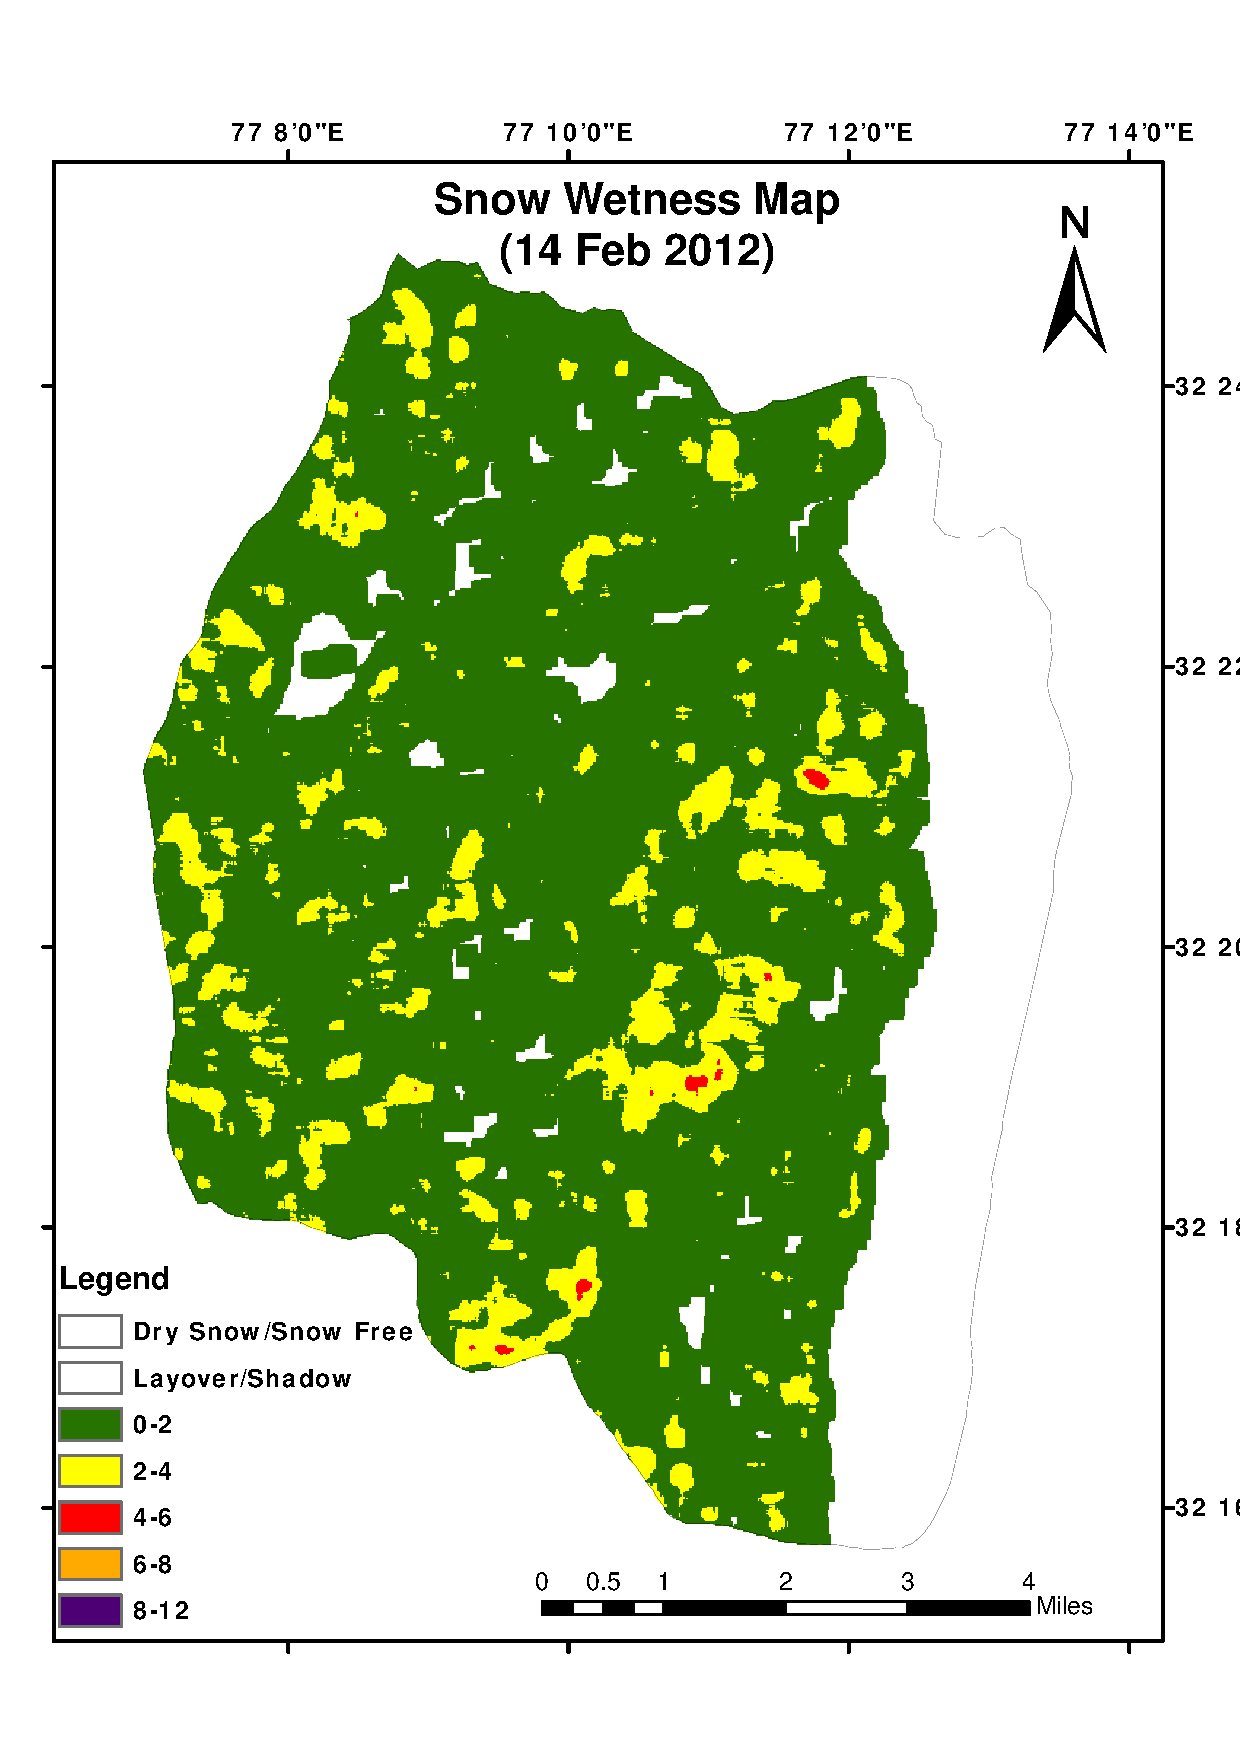
\includegraphics[width=0.45\textwidth]{Figures/14Feb2012}}
	\subfloat[]{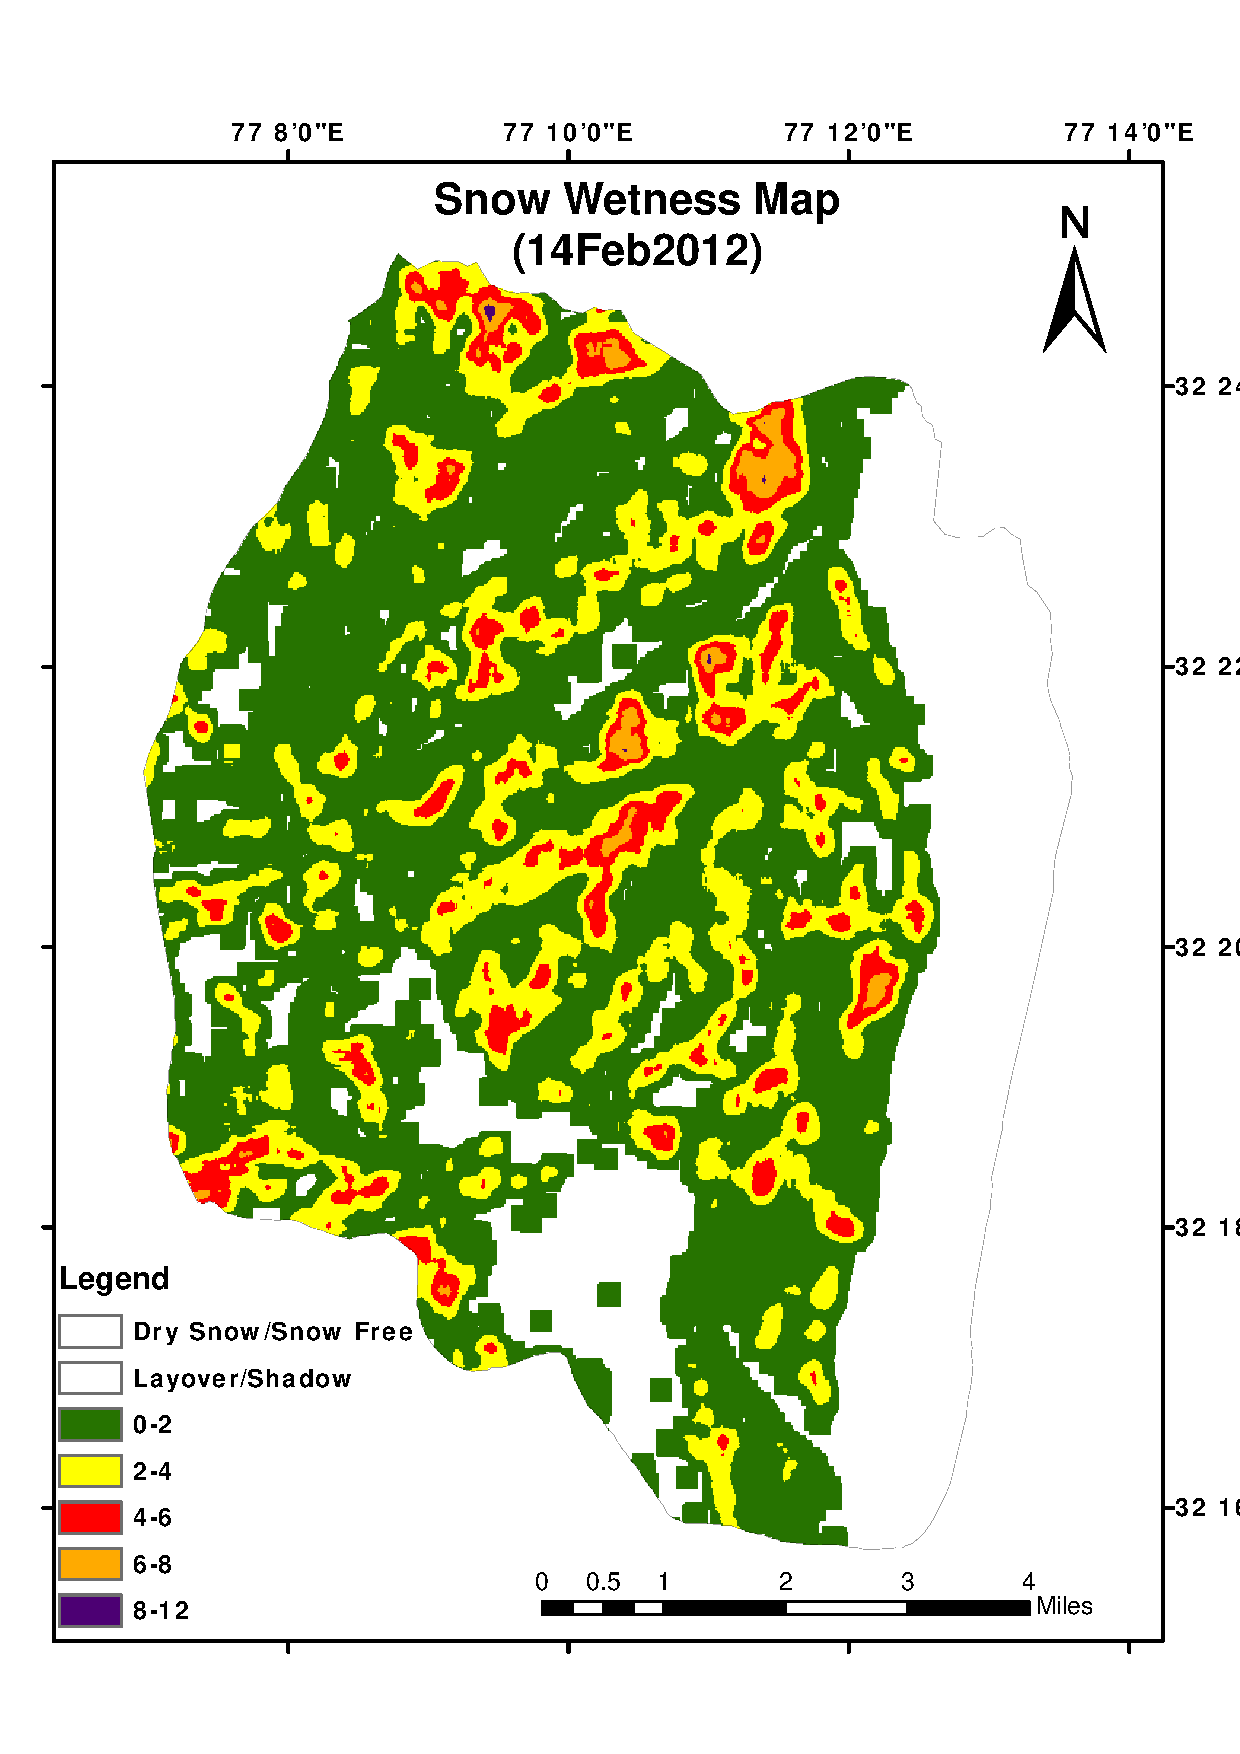
\includegraphics[width=0.45\textwidth]{Figures/14Feb2012_shi}}
	\caption[Comparison of the proposed and Shi~-Dozier snow wetness maps of 14 Feb. 2012 Radarsat-2 data] {Comparison of the snow wetness maps (in $\%$ volume) derived from (a) the proposed and (b) the Shi~-Dozier method. The white blank portion on the right hand side of the map is due to out of data coverage.}
	\label{fig:proposed_shi_dozier_results}
\end{figure}

The snow wetness map for 7 Feb 2012 (Figure~\ref{fig:proposed_results_fullpol1}(a)) data shows that the wetness is in the range of 2--3$\%$ around the Bahang observatory. During this descending pass acquisition, the in-situ measurements were collected around the Bahang observatory and the temperature was recorded around -~2$^\circ$C. The estimated wetness values have a decent concurrence with the field data collected in near-real time with the satellite pass. In the following year, the effective snow wetness was estimated for 6 and 8 Feb 2013 datasets. The snow wetness map derived from the proposed model for the 6 Feb data (Figure~\ref{fig:proposed_results_fullpol1}(b)), shows that the wetness over the Bahang observatory region is around 3--6$\%$ with the maximum temperature of 4$^\circ$C. The wetness is around 1--3$\%$ over the Solang and the Dhundhi observatories where the maximum temperatures were recorded at 1.5$^\circ$C and 1$^\circ$C respectively along with a fresh snowfall on that day. 
\begin{figure}[!thpb]
	\centering
	\subfloat[]{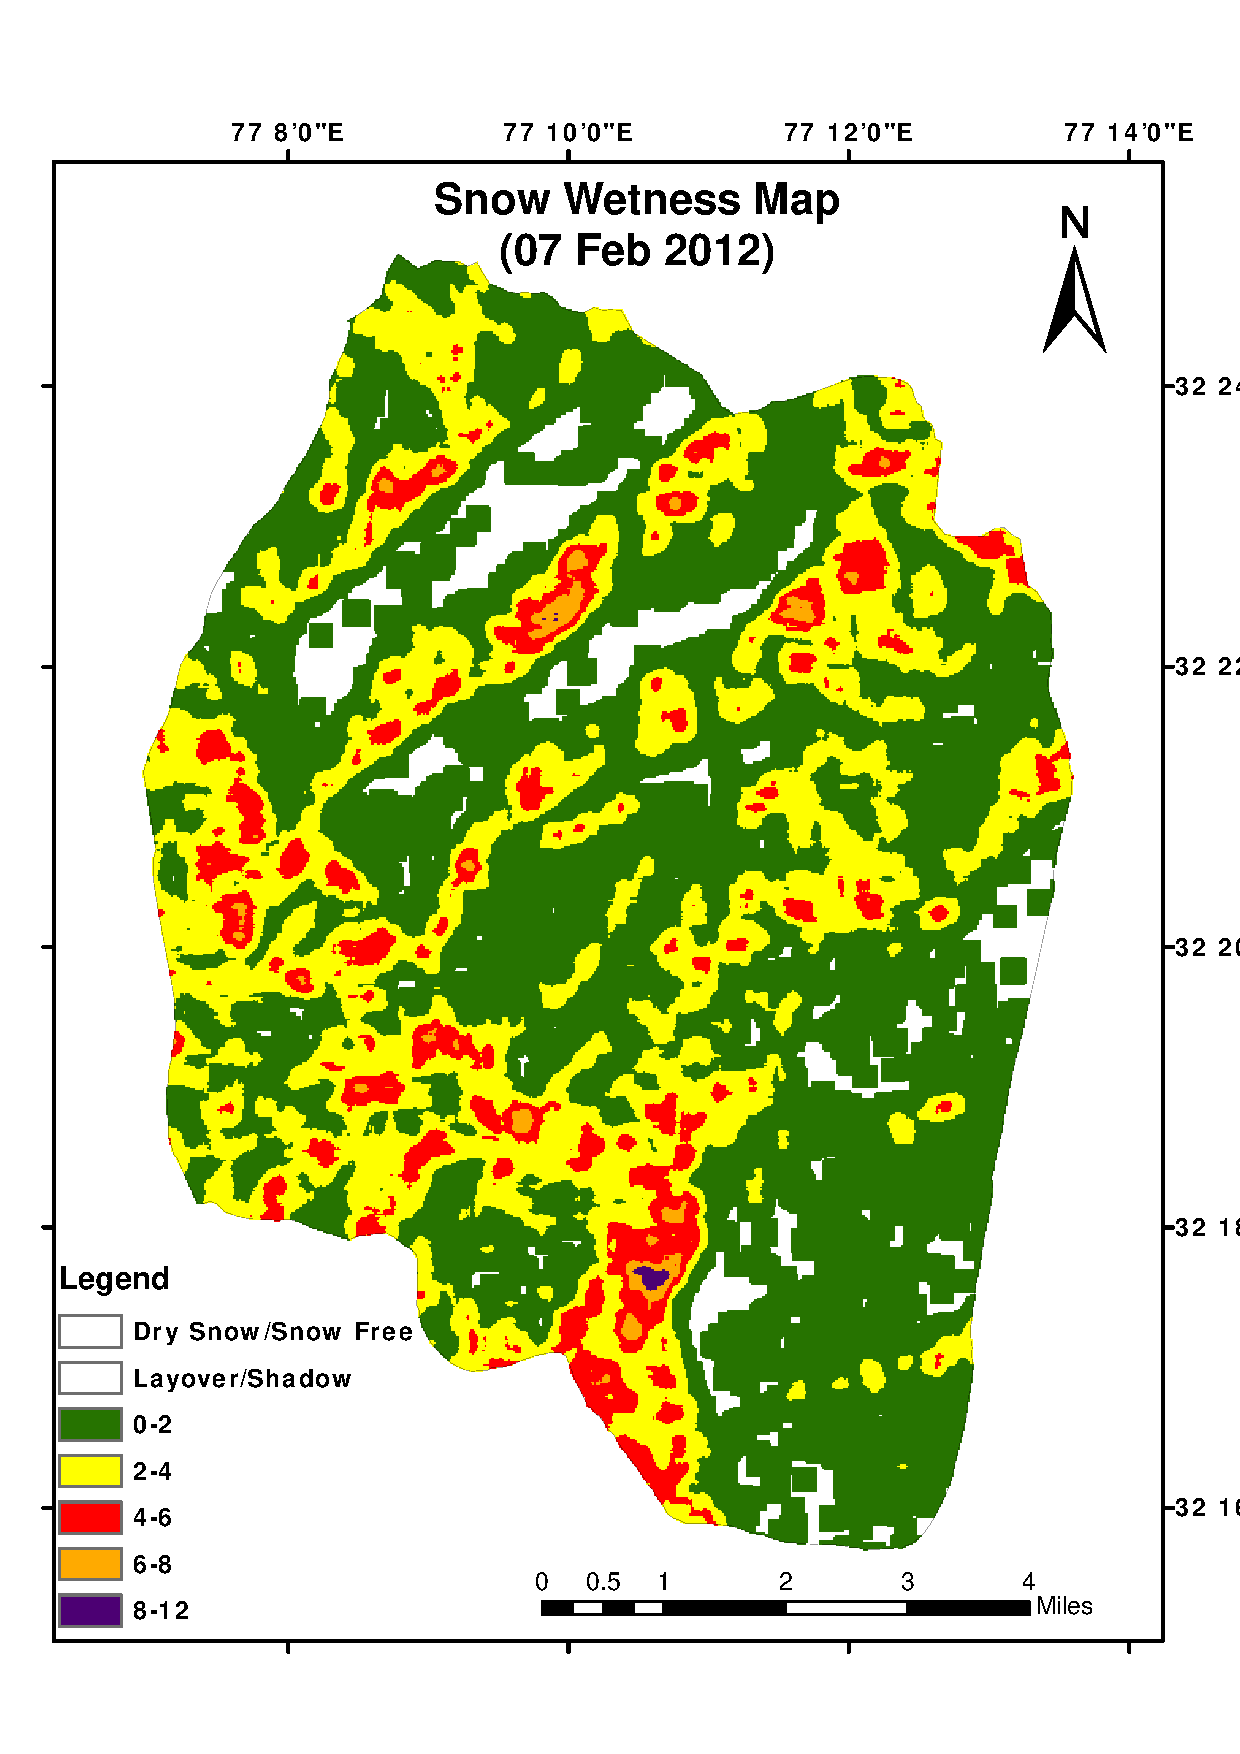
\includegraphics[width=0.45\textwidth]{Figures/07Feb2012}} 
	\subfloat[]{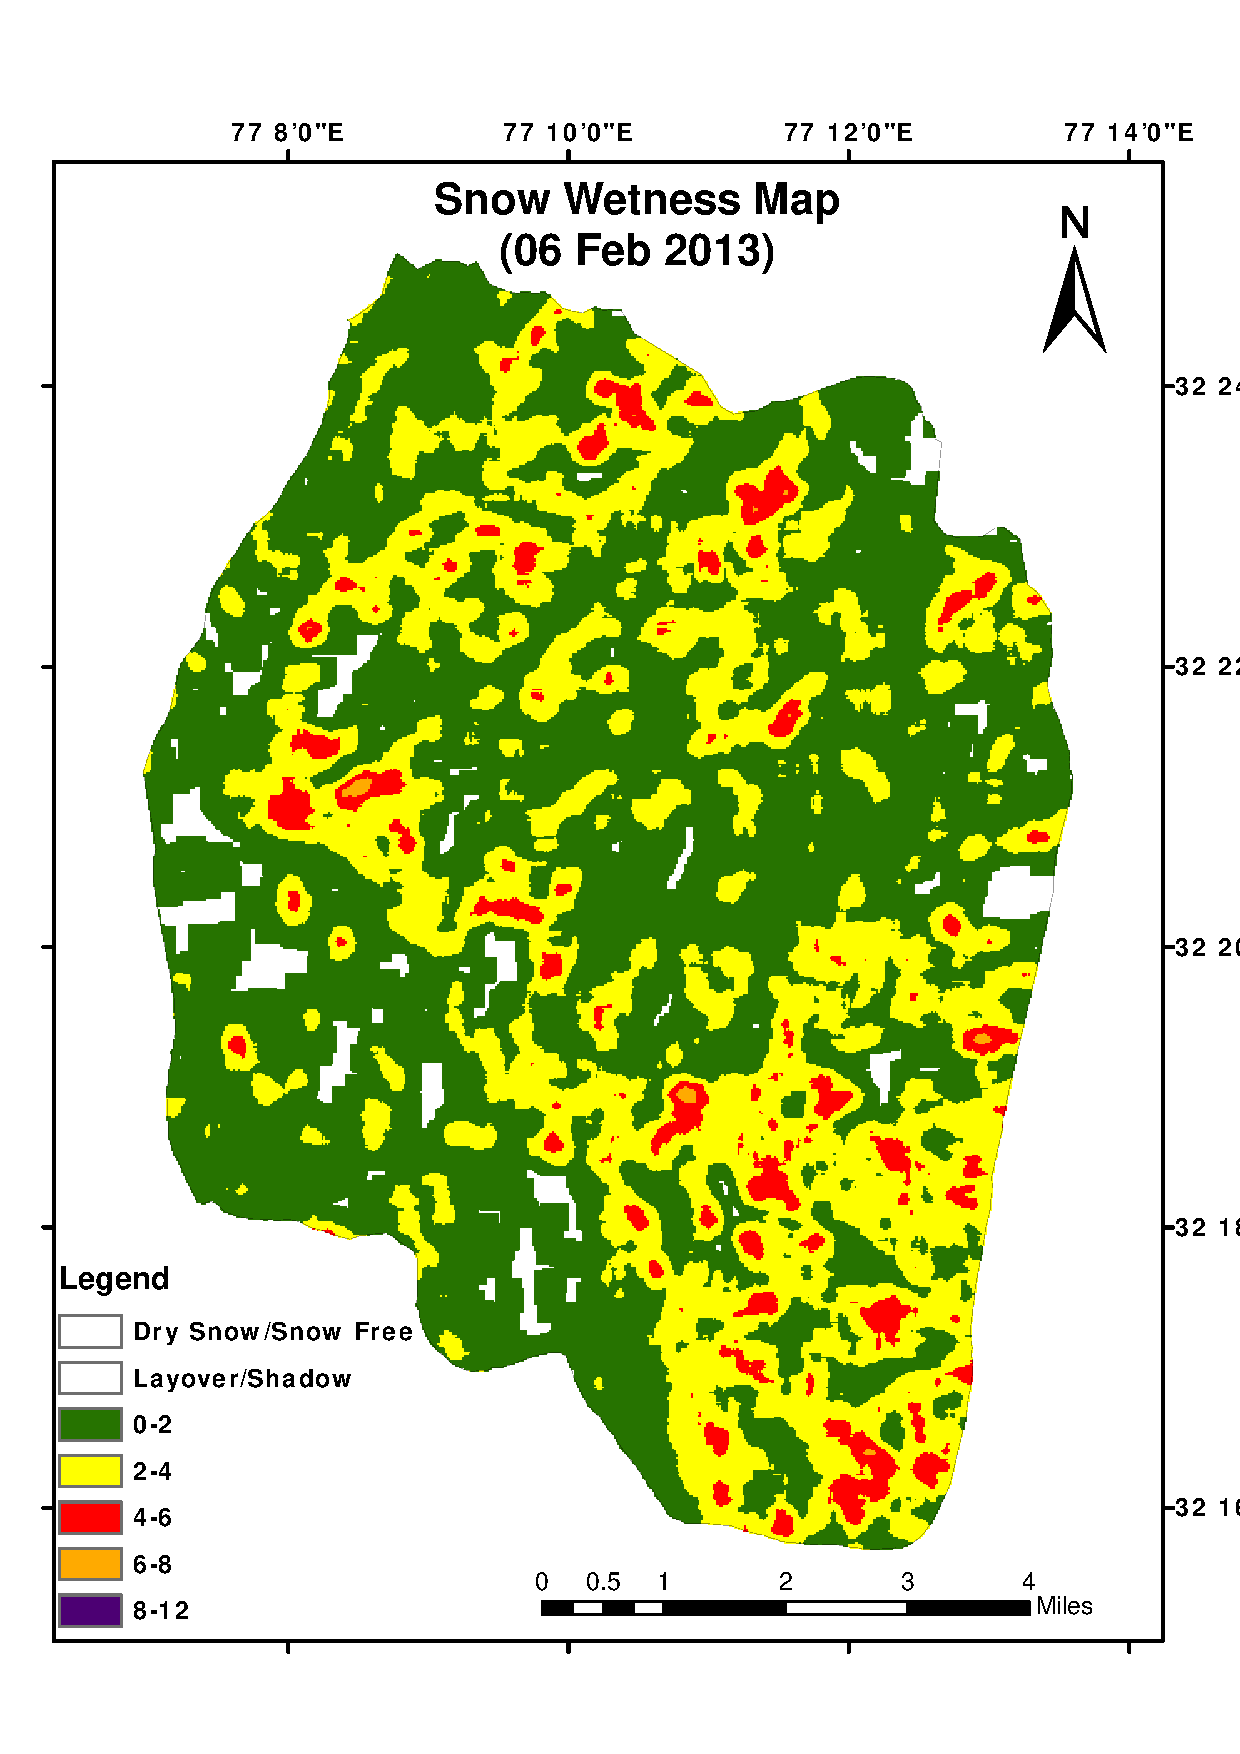
\includegraphics[width=0.45\textwidth]{Figures/06Feb2013}} 
	\caption [Snow wetness maps of 07 Feb. 2012 and 06 Feb. 2013 Radarsat-2 data]{Snow wetness maps (in $\%$ volume) derived from the proposed model.} 
	\label{fig:proposed_results_fullpol1}
\end{figure}

The effective snow wetness map for 18 Feb 2014 is shown in Figure~\ref{fig:proposed_results_fullpol2}(a) which is derived using the weighted average of surface and volume snow wetness maps. It shows that the wetness is in the range of 3--6$\%$ over the study area. The maximum temperature for the day was recorded around 17$^\circ$C, 14$^\circ$C and 8$^\circ$C in the Bahang, Solang and Dhundi observatories, respectively. Due to this high temperature there was a melting of 6 cm, 11 cm and 7 cm of snow within a span of less than 12 hours recorded at the three observatories respectively. This  can be clearly seen in the effective snow wetness map Figure~\ref{fig:proposed_results_fullpol2}(a) which is obtained from the surface (6--9$\%$) and the volume (3--8$\%$) snow wetness maps. This may be due to the melting of snow surface which subsequently percolates into the snowpack, thereby increasing the volume wetness.

\begin{figure}[!thpb]
	\centering
	\subfloat[]{\includegraphics[width=0.45\textwidth]{Figures/18Feb2014}}
	\subfloat[]{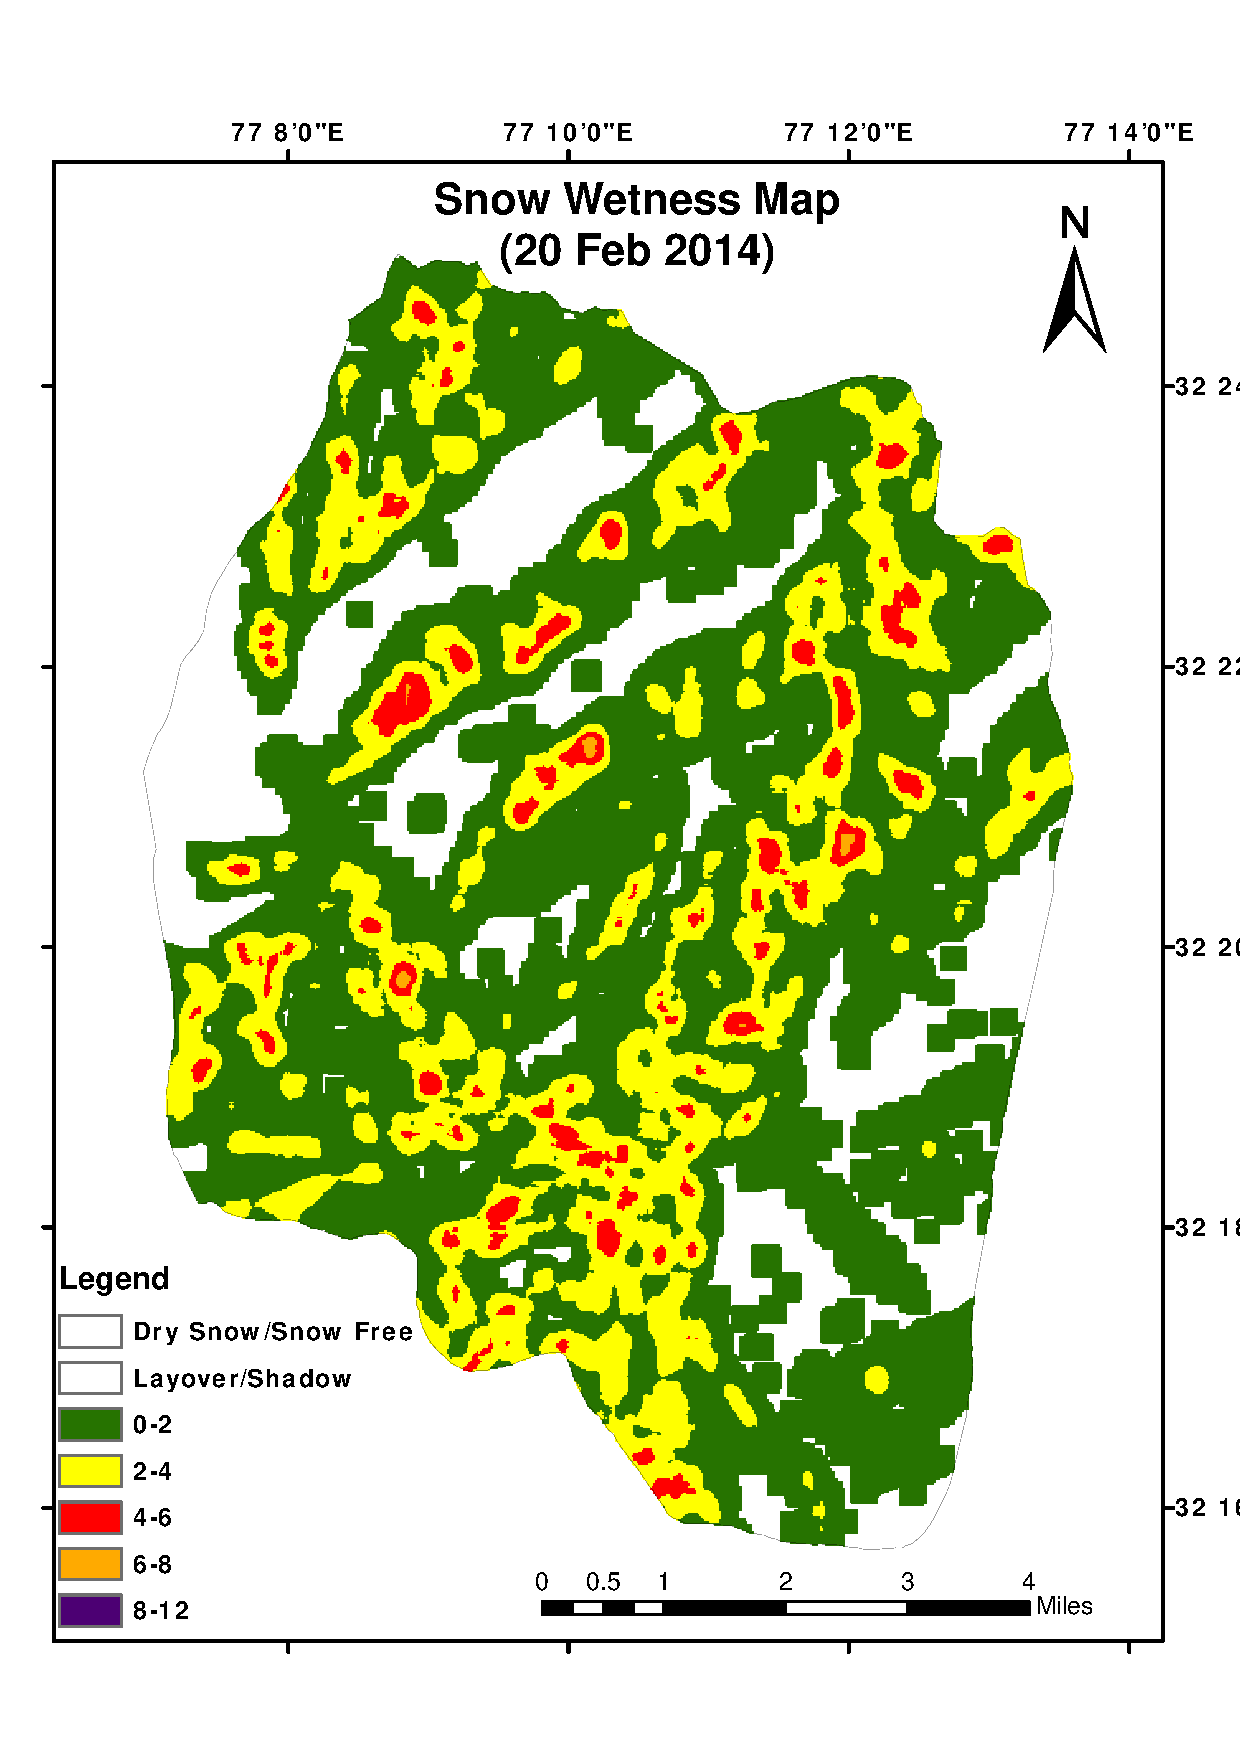
\includegraphics[width=0.45\textwidth]{Figures/20Feb2014}}
	\caption [Snow wetness maps of 18 Feb. 2014 and 20 Feb. 2014 Radarsat-2 data]{Snow wetness maps (in $\%$ volume) derived from the proposed model. RADARSAT-2 Data and Products ©MacDonald, Dettwiler and Associates Ltd. (2014) $–$ All Rights Reserved. RADARSAT is an official trademark of the Canadian Space Agency} 
	\label{fig:proposed_results_fullpol2}
\end{figure}

A total of 40 in-situ measurements were collected in near-real time with the satellite data for three consecutive years to validate the proposed snow wetness estimation algorithm. The snow wetness estimated by the proposed and the Shi-Dozier algorithms along with in-situ measurements are plotted in Figure~\ref{fig:validation_plot_fullpol_SW}(a) and (b) respectively. Particularly for low wetness condition ($<$ 3.5$\%$), the proposed model closely follows the in-situ measurements than the Shi-Dozier method. However, for most of the cases the Shi-Dozier method overestimates the snow wetness. The three in-situ measurements on 7 Feb 2012 over the Dhundi observatory were collected around six hours after the satellite pass. Due to this, the overestimation in the snow wetness is clearly seen in Figure~\ref{fig:validation_plot_fullpol_SW}(a) marked within the black box.
\begin{figure}[!thpb]
	\centering
	\subfloat[]{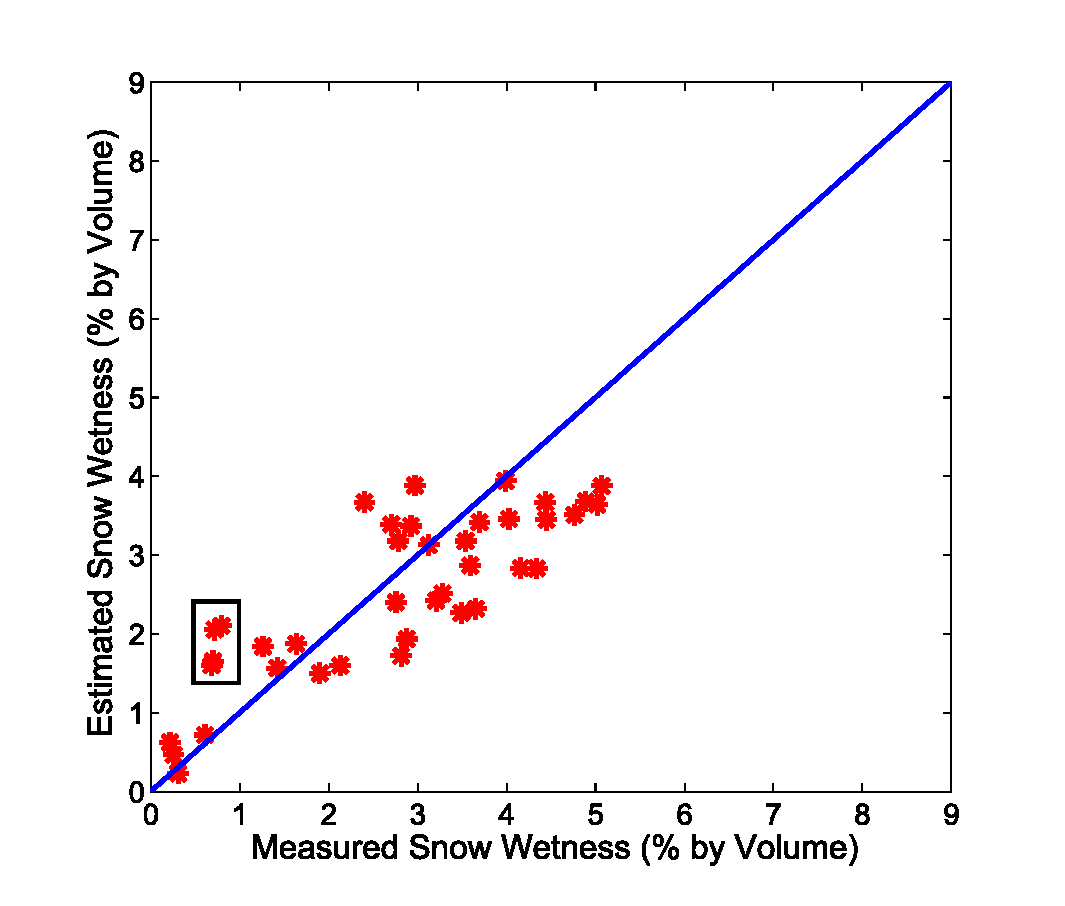
\includegraphics[width=0.45\textwidth]{Figures/validation_plot_proposed}}
	\subfloat[]{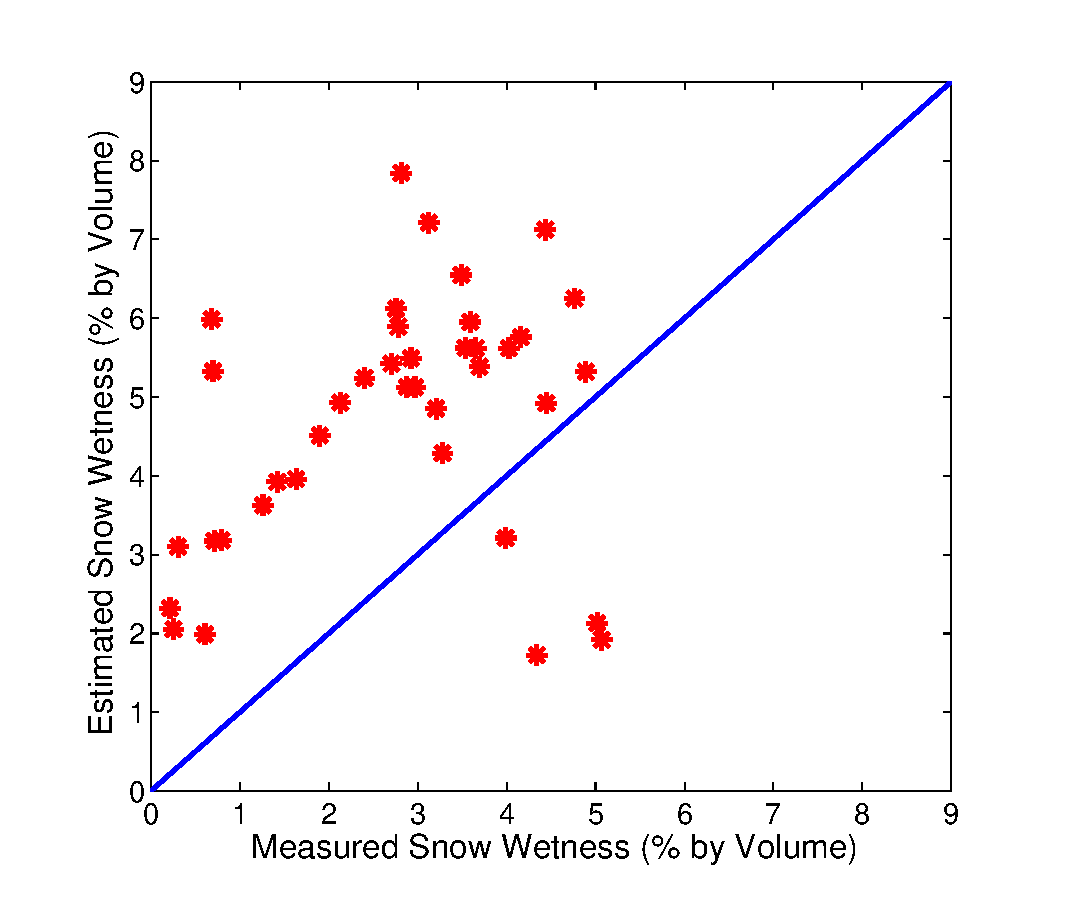
\includegraphics[width=0.45\textwidth]{Figures/validation_plot_shi}}
	\caption [Validation of the snow wetness estimation methods from full polarimetry SAR data]{Comparison of the estimated snow wetness by (a) the newly proposed and (b) the existing Shi~-Dozier methods along with in-situ measurements.} 
	\label{fig:validation_plot_fullpol_SW}
\end{figure}
\FloatBarrier
\section{Snow surface dielectric constant}
\FloatBarrier
\begin{figure*}[!htbp]
	\centering
	\subfloat[]{\includegraphics[width=0.45\textwidth]{Figures_SSD/7Feb2012}}
	\subfloat[]{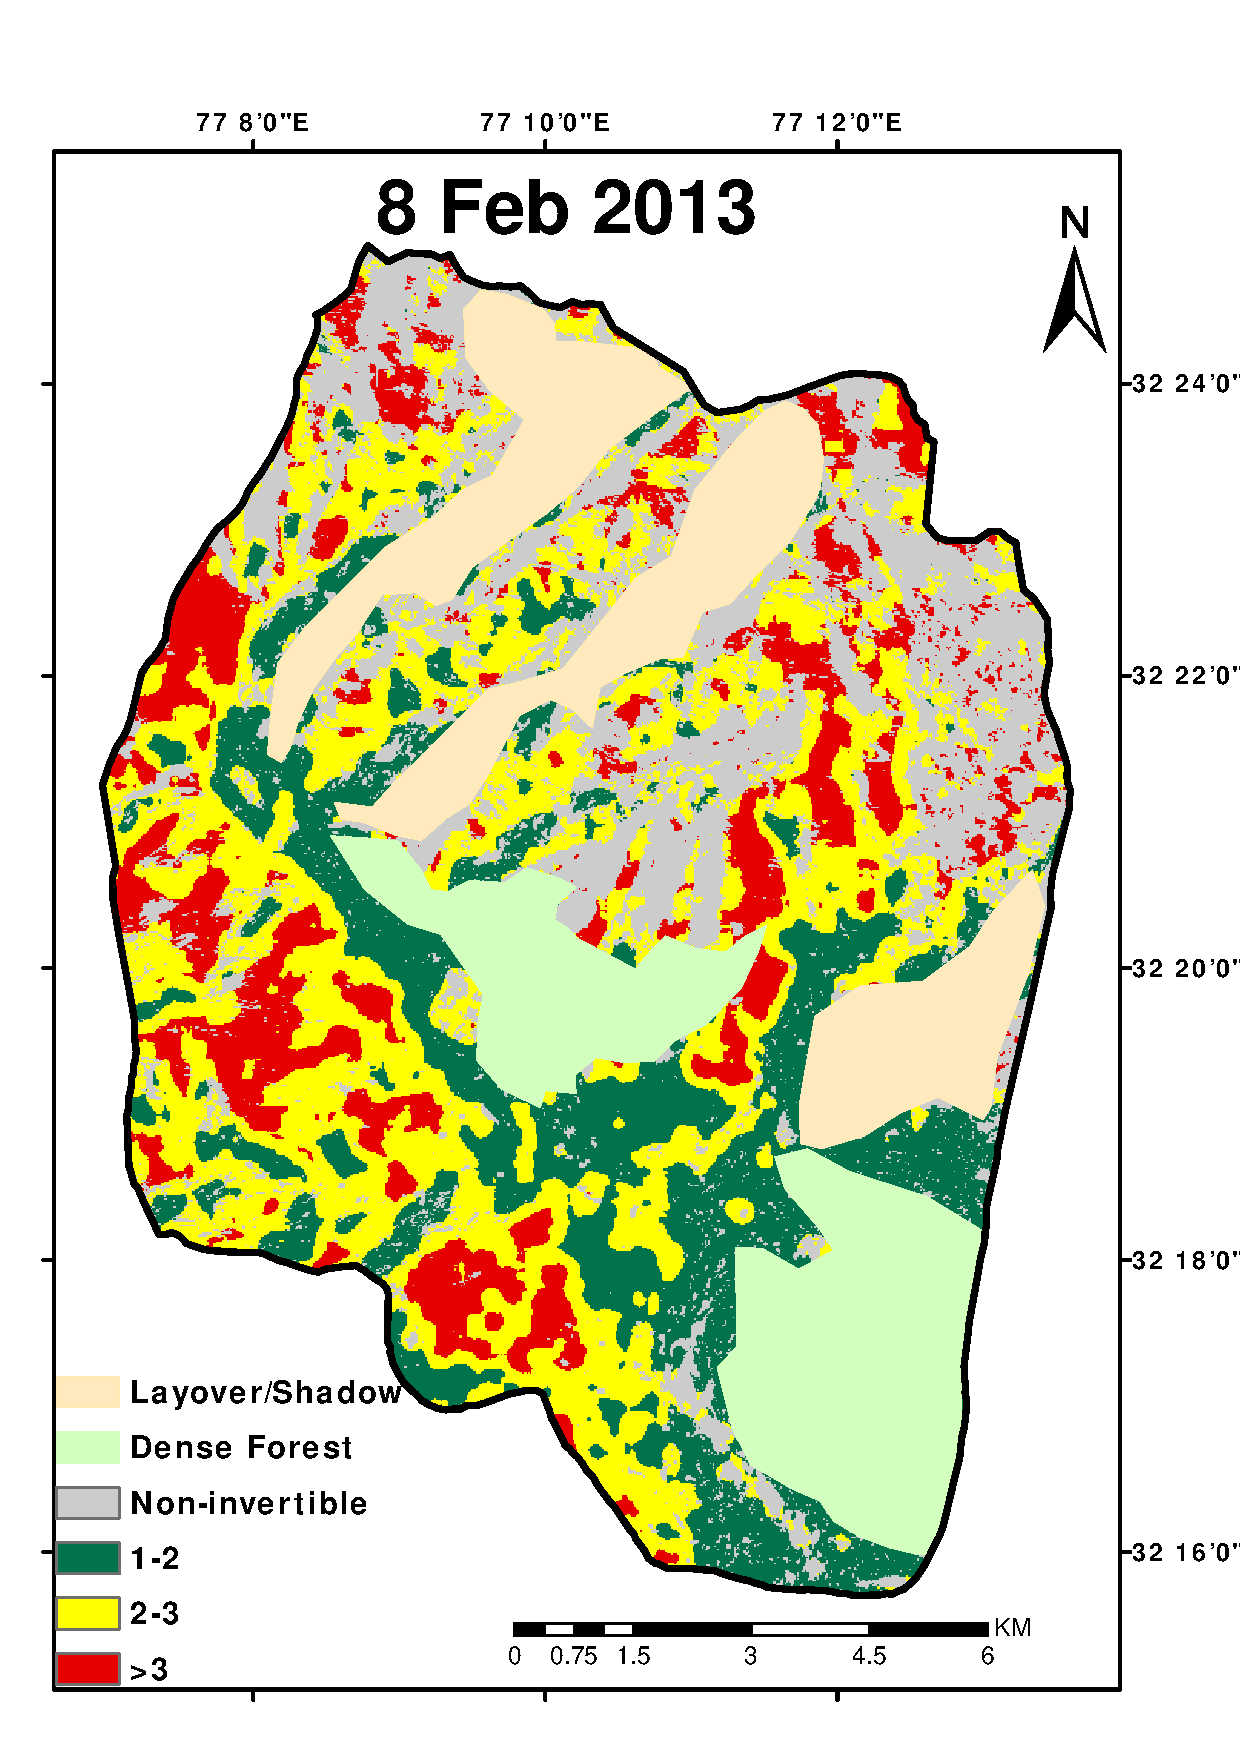
\includegraphics[width=0.45\textwidth]{Figures_SSD/8feb2013}}\\
	\subfloat[]{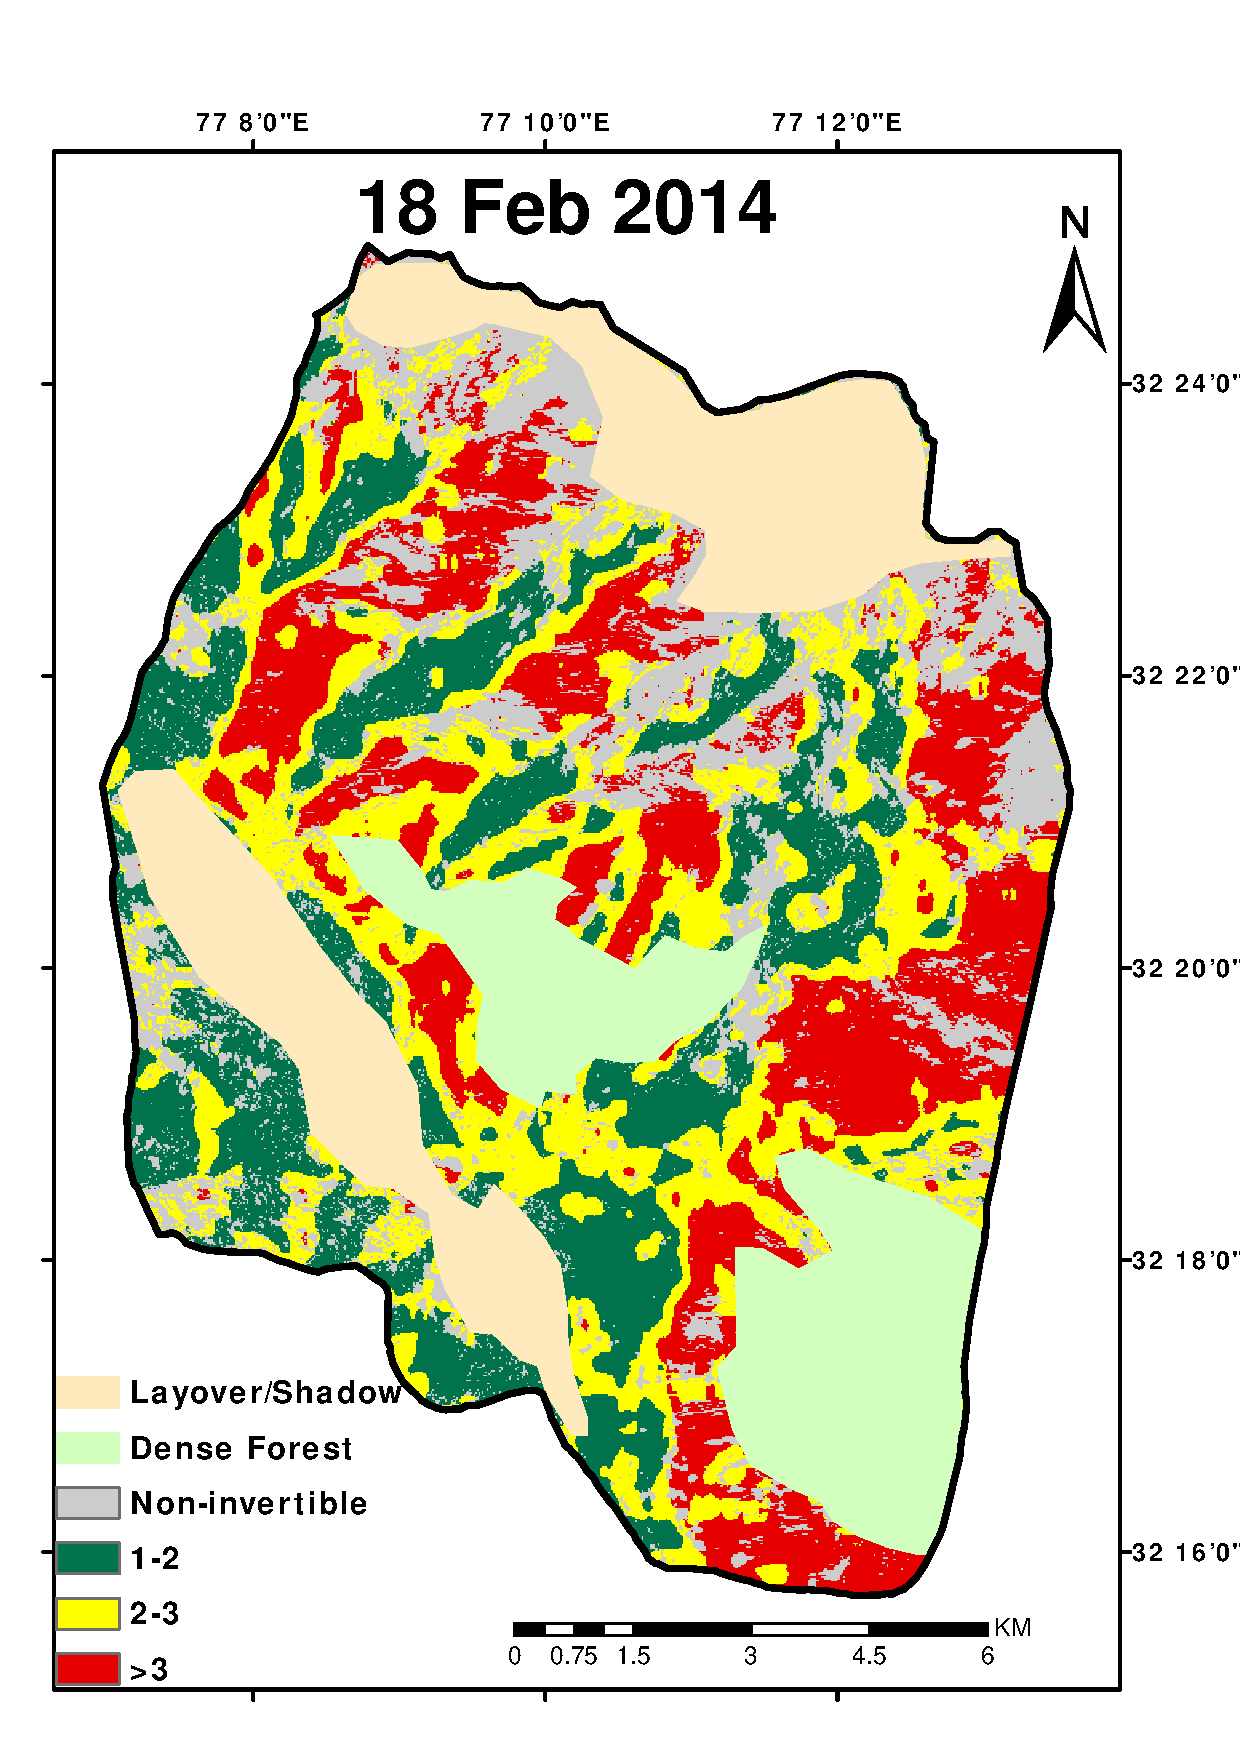
\includegraphics[width=0.45\textwidth]{Figures_SSD/18feb2014}}
	\caption[Snow surface dielectric constant maps]{Temporal snow surface dielectric constant maps estimated over the Manali-Dhundi area for three consecutive winters. (For figure (c): RADARSAT-2 Data and Products ©MacDonald, Dettwiler and Associates Ltd. (2014) $-$ All Rights Reserved. RADARSAT is an official trademark of the Canadian Space Agency)} 
	\label{fig:SSD_results}
\end{figure*}

The proposed algorithm for the estimation of snow surface dielectric constant~(\cref{sec:3.3}) is applied to the fine resolution full-polarimetric Radarsat-2 C-band SAR data acquired over the Manali-Dhundi area in Himachal Pradesh, India~(\cref{sec:4.2.1}). The 3$\times$3 coherency matrix was generated from the single-look complex data. A multi-looking factor of 3 in the range and 4 in the azimuth direction was used to make a pixel square and the Lee-Refined filter was applied to remove the speckle noise. The local incidence angle map is generated while performing the Range Doppler terrain correction using the 30~m SRTM DEM and the Layover/Shadow areas were masked. After these pre-processing, the range and azimuthal pixel spacing of the image was approximately 20~m (19.7~m$\times$20.9~m) respectively. Field campaigns were conducted to collect near-real time in-situ measurements using the snowfork instrument and a hand held GPS with all the three Radarsat-2 data acquisitions for three consecutive winter seasons from 2012 to 2014~(Table~\ref{table:data acquisition}).

%\begin{figure*}[!h]
%	\centering
%	\subfloat[\label{Fig:Snow_surf_diel_7Feb2012}]{\includegraphics[width=0.4\columnwidth]{Figures_SSD/7Feb2012}} \hspace{1mm}
%	\subfloat[\label{Fig:Snow_surf_diel_8Feb2013}]{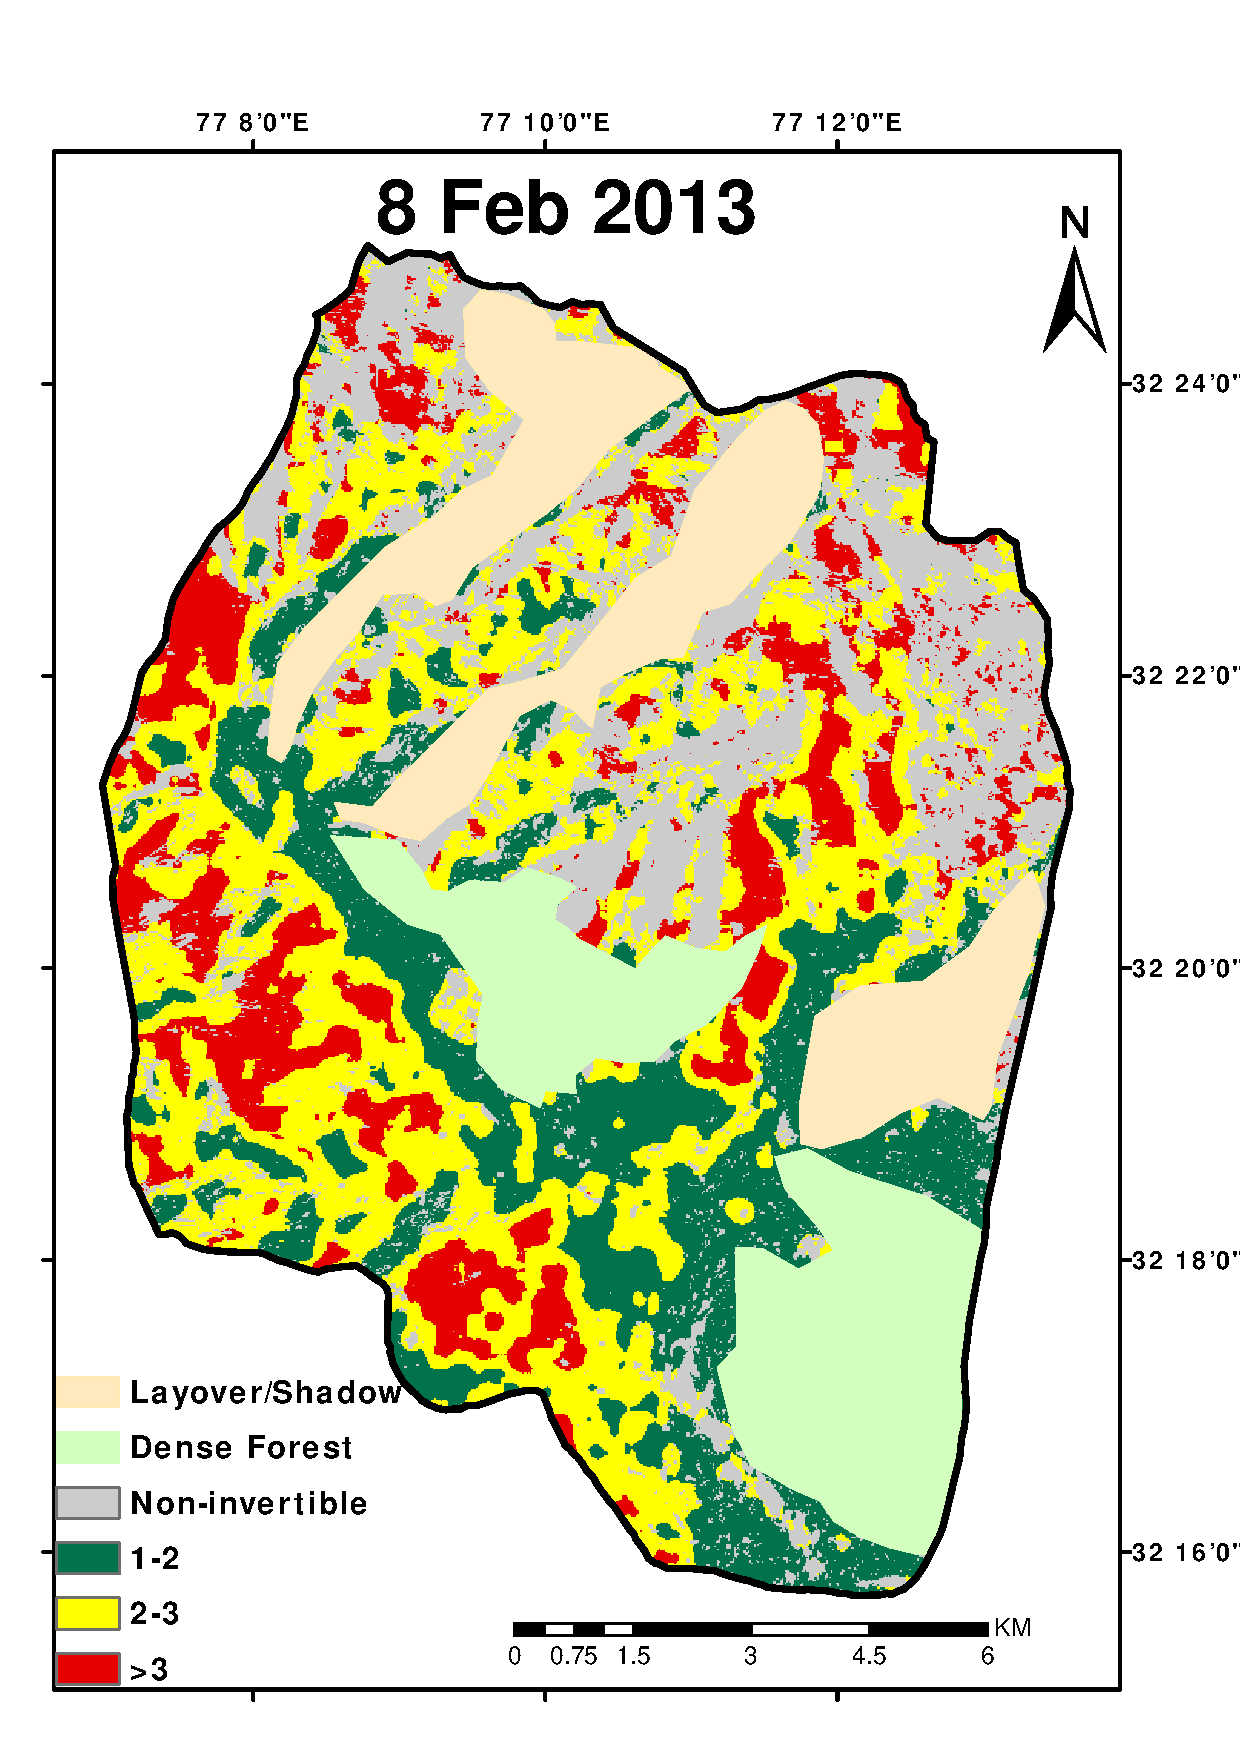
\includegraphics[width=0.4\columnwidth]{Figures_SSD/8feb2013}} \hspace{1mm}
%	\subfloat[\label{Fig:Snow_surf_diel_18Feb2014}]{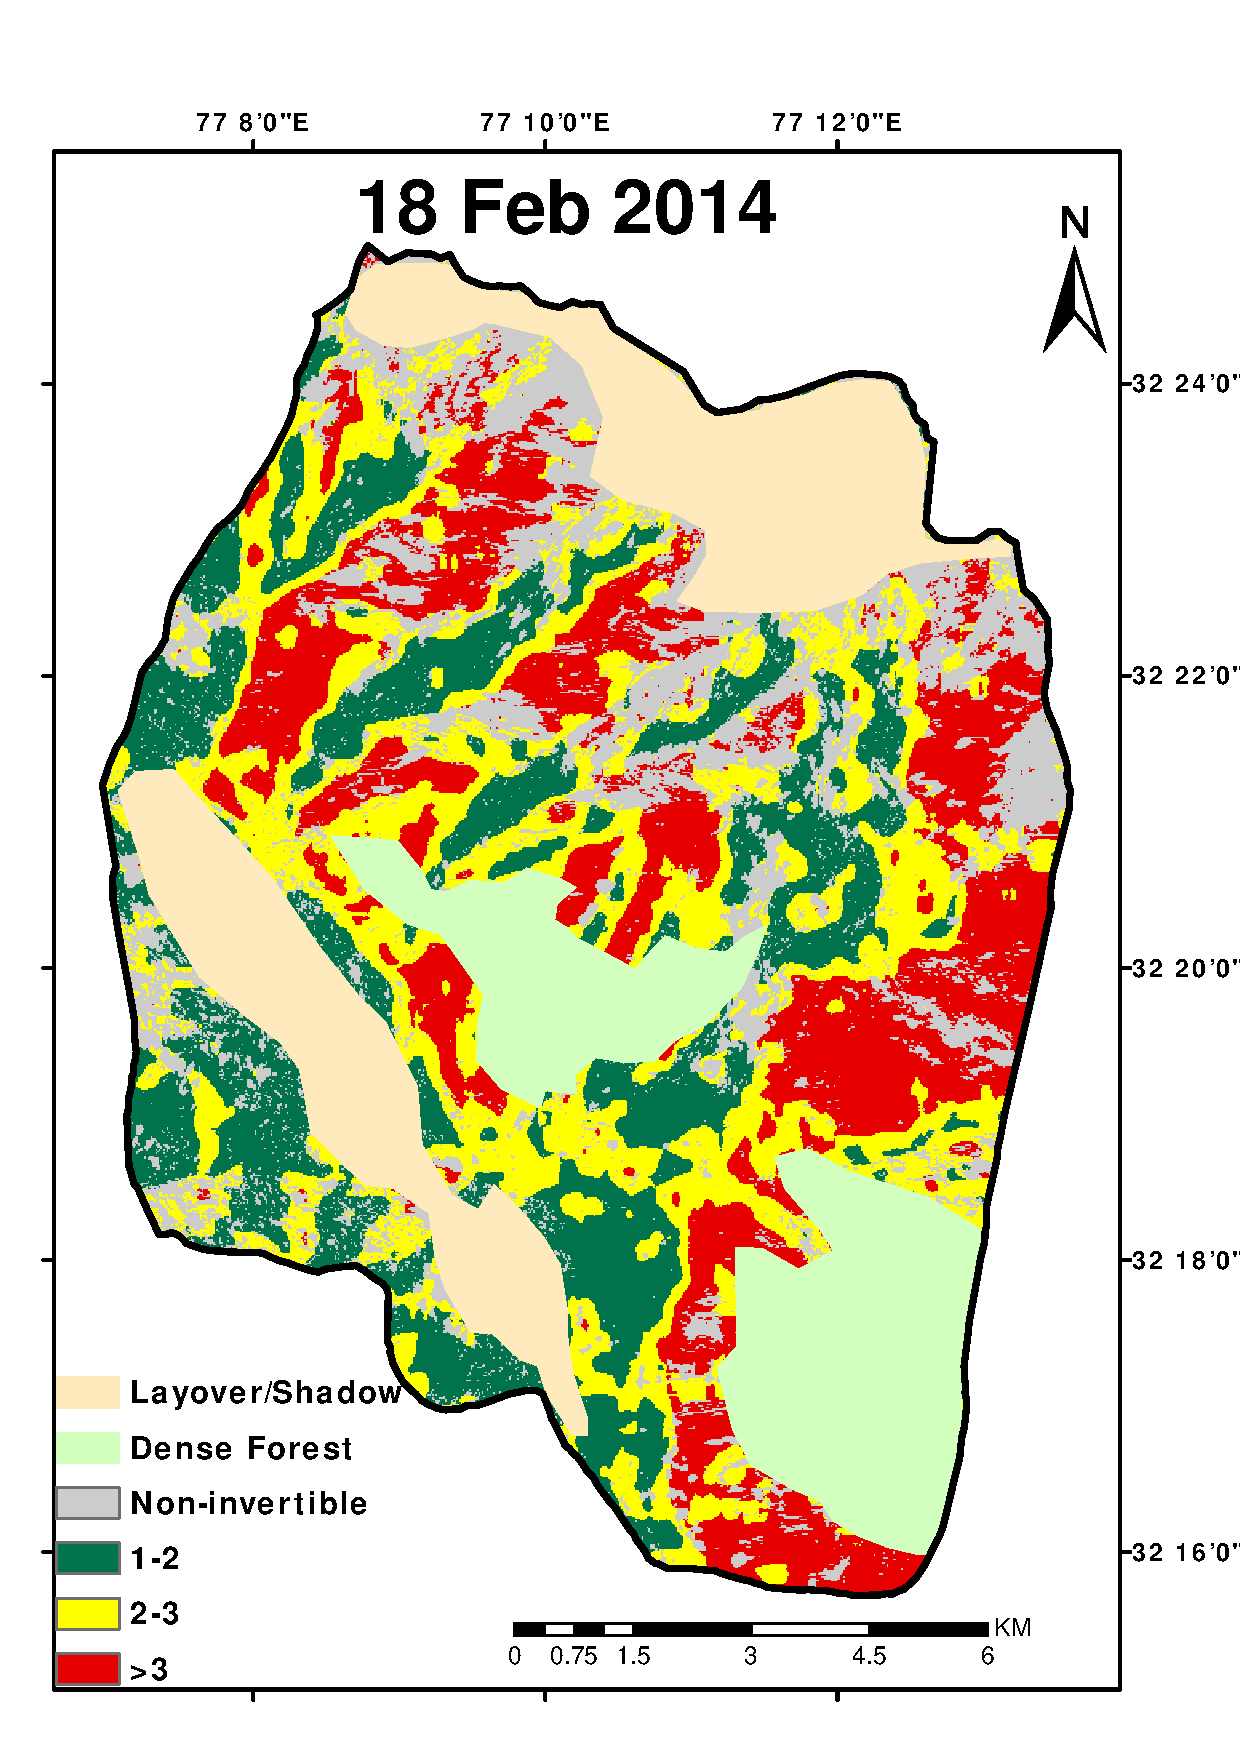
\includegraphics[width=0.4\columnwidth]{Figures_SSD/18feb2014}} 
%	\caption{Temporal snow surface dielectric constant maps estimated over the Manali-Dhundi area for three consecutive winters (\protect\subref{Fig:Snow_surf_diel_7Feb2012}, \protect\subref{Fig:Snow_surf_diel_8Feb2013}, \protect\subref{Fig:Snow_surf_diel_18Feb2014}).}
%	\label{fig:results_2}
%\end{figure*}	


%\begin{figure*}[!h]
%	\centering
%	\subfloat[\label{Fig:29Jan2015}]{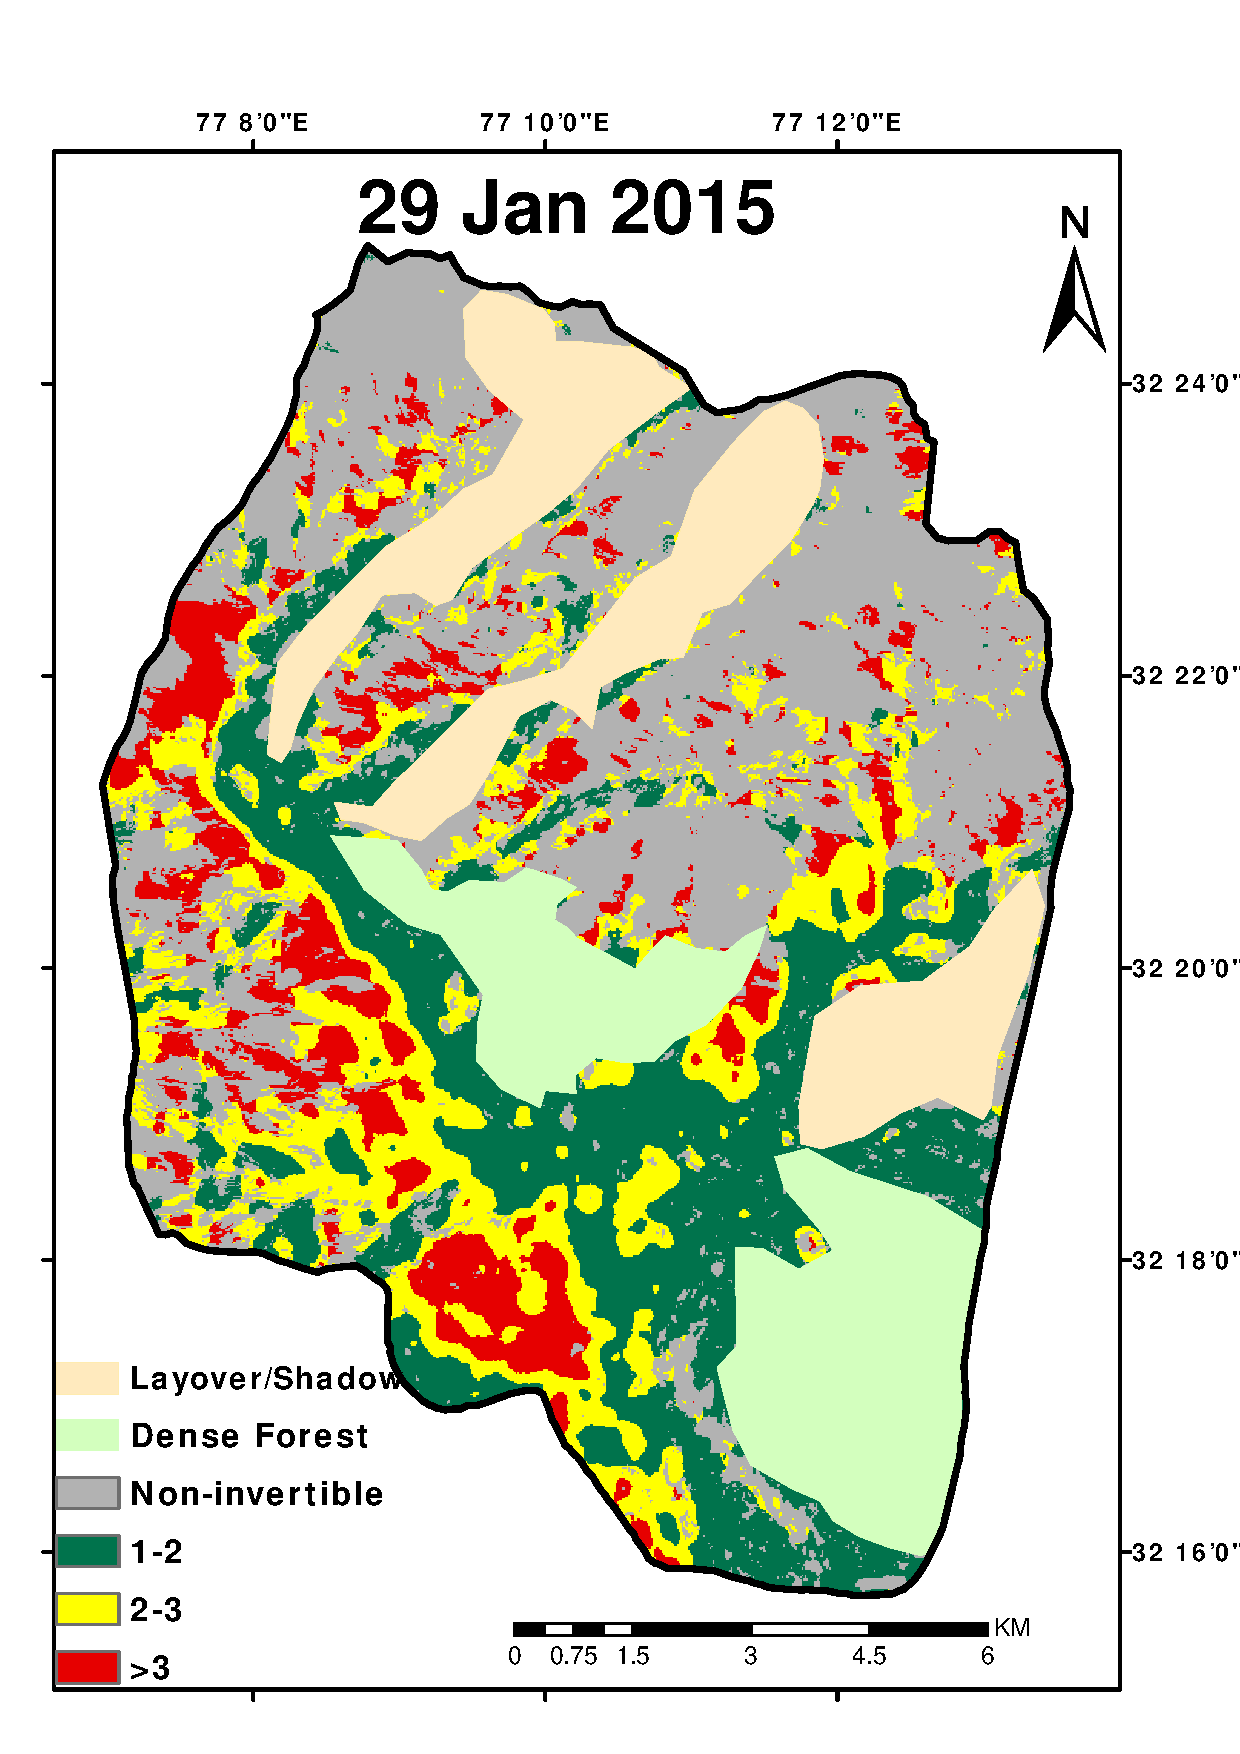
\includegraphics[width=0.49\columnwidth]{Figures_SSD/SSD_29Jan15}} \hspace{1mm}
%	\subfloat[\label{Fig:22Feb2015}]{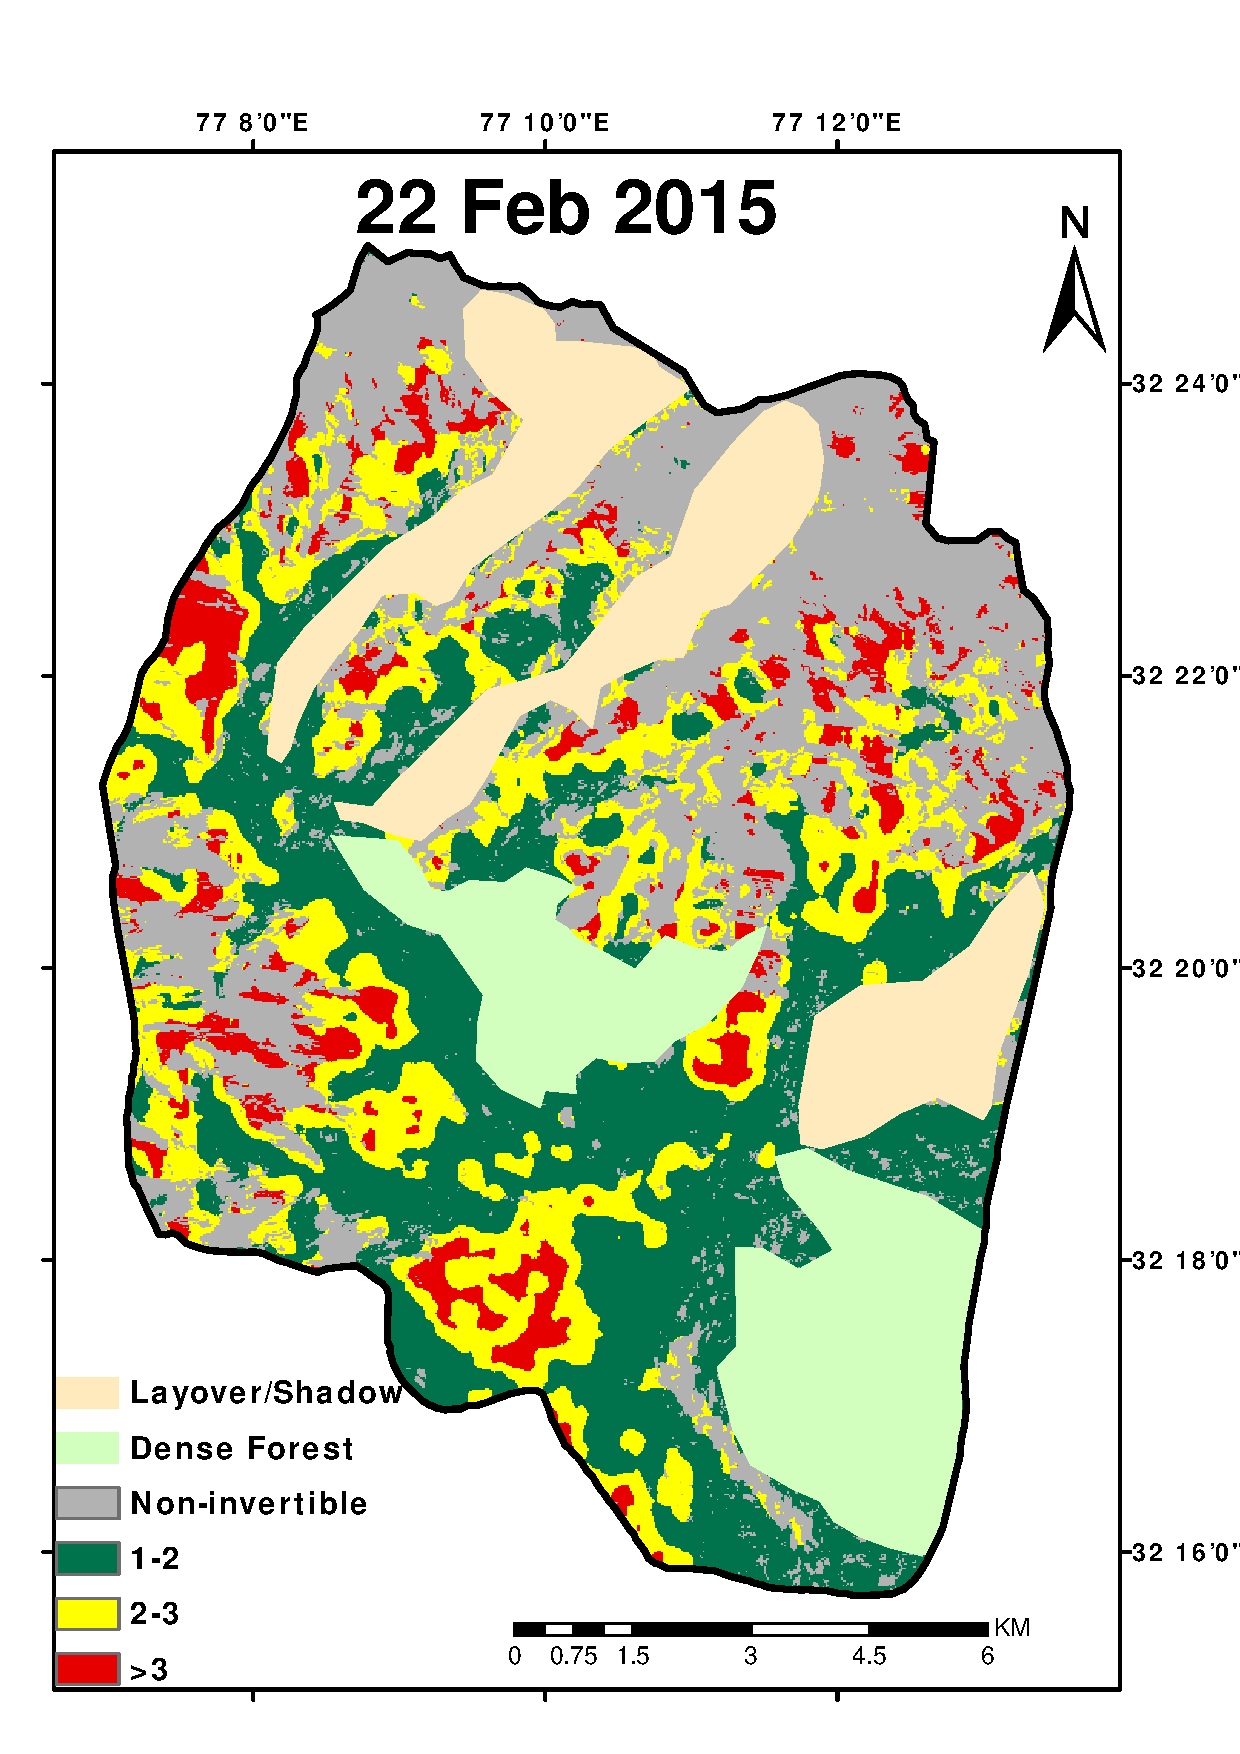
\includegraphics[width=0.49\columnwidth]{Figures_SSD/SSD_22Feb15}} 
%	\hspace{1mm}
%	\subfloat[\label{Fig:18Mar2015}]{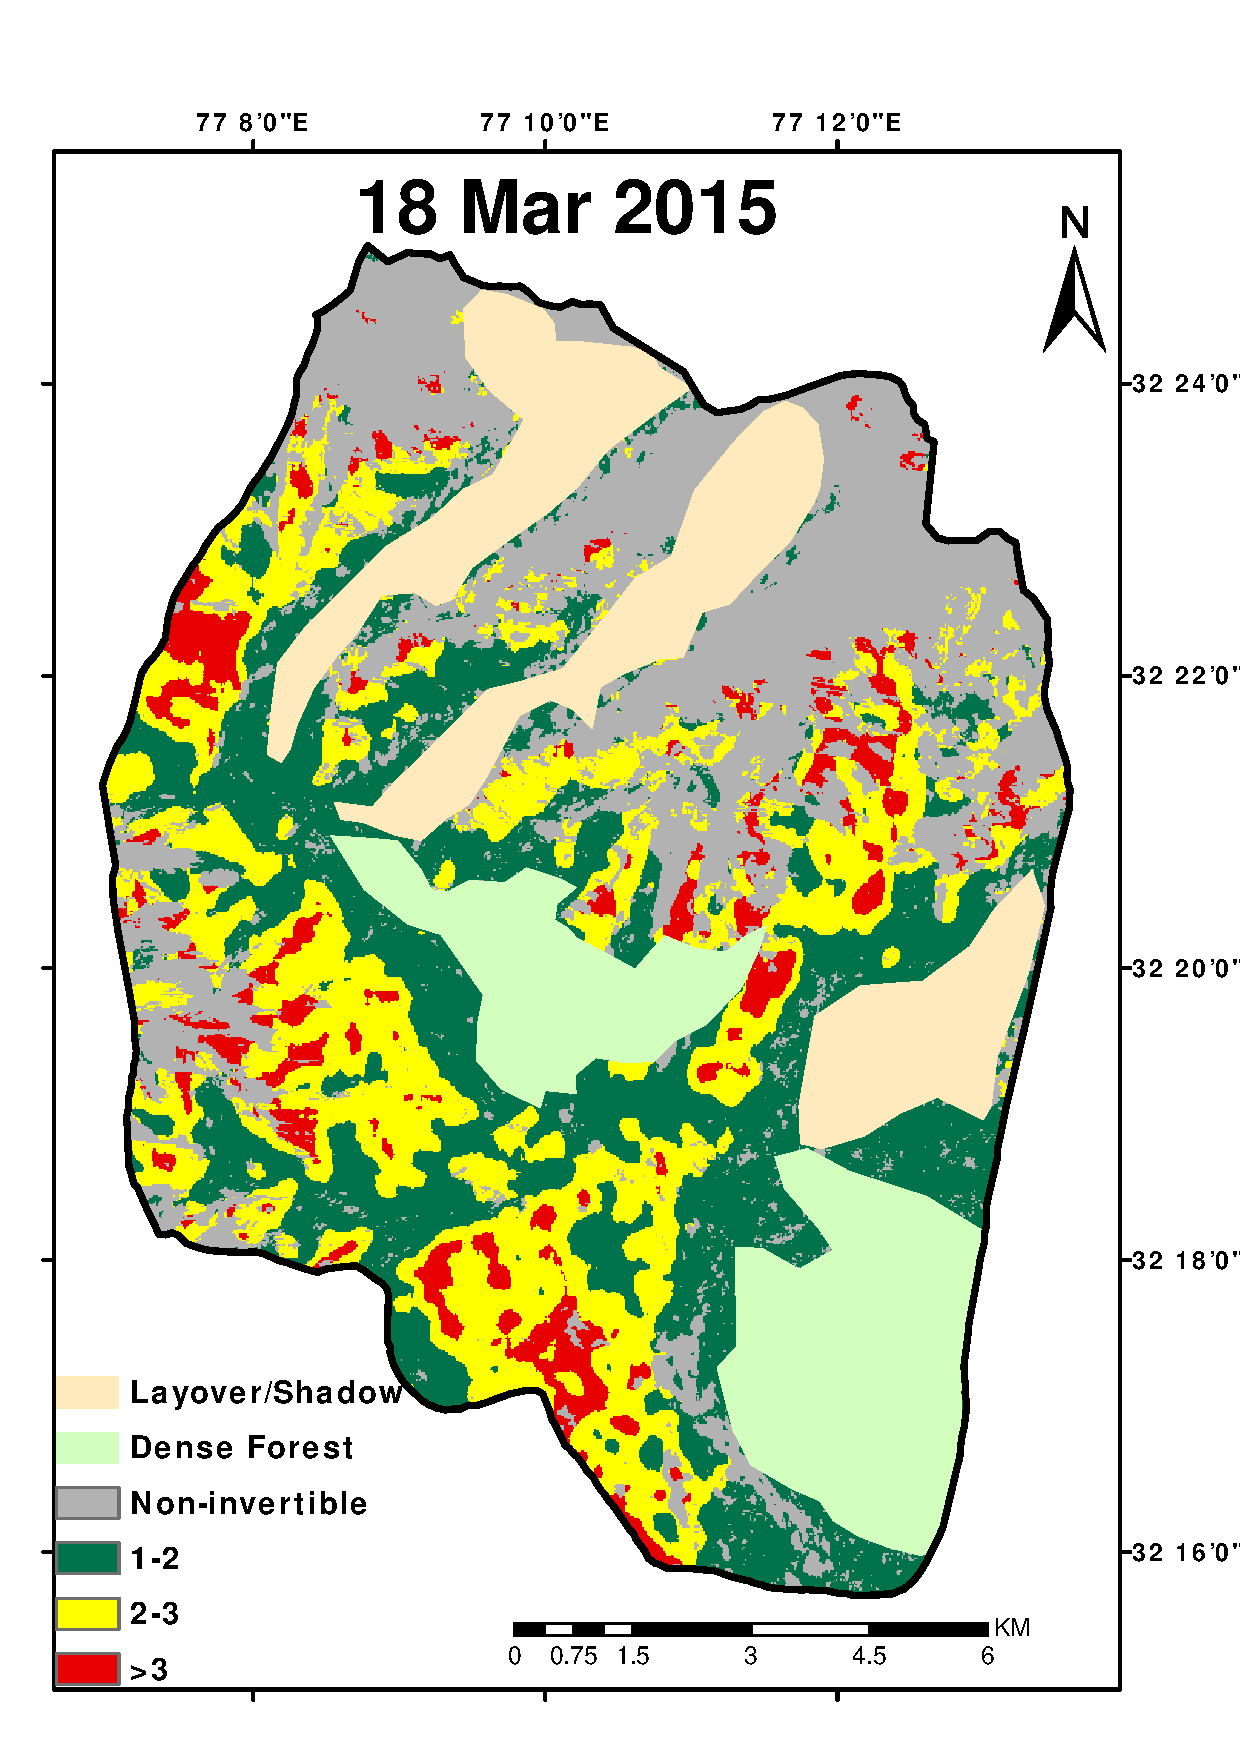
\includegraphics[width=0.49\columnwidth]{Figures_SSD/SSD_18Mar15}} 
%	\caption{Multi-temporal snow surface dielectric constant maps in a season over the study area}
%	\label{fig:Multi_temporal_SSD}
%\end{figure*}
Using the criteria of $m_{E}^{\mbox{\scriptsize opt}} > 0.5$, it is observed that there is approximately $9-10\%$ increase in the number of invertible pixels compared to the original data $(\langle[{\mathbf{T}}]\rangle)$ for all the data sets used in this study. However, it can be observed that in most areas including higher altitude, $p_{max} > 0.5$ as shown in Figure~\ref{fig:results_1}(b), whereas it is observed that $m_{E}^{\mbox{\scriptsize opt}} < 0.5$ over high altitude regions as shown for 8 Feb. 2013 data in Figure~\ref{fig:results_1}(a). This can be attributed to the fact that: (1). $m_{E}^{\mbox{\scriptsize opt}}$ is obtained in HV basis by minimizing the $T_{33}$ component of the $\langle[\mathbf{T}]\rangle$ matrix unlike $p_{max}$ which is computed over all possible basis $(\chi_{t},\psi_{t})$. (2). Specifically over high altitude regions, $\chi_{t}^{\mbox{\scriptsize opt}} \approx \pm 45^\circ$ (circular polarization) for the corresponding high values of $p_{max}$. This suggests that over these regions $p_{max}$ is obtained for a circular basis (right or left) whereas $m_{E}^{\mbox{\scriptsize opt}}$ is always obtained in the linear HV basis.

Moreover, it can also be observed that even though $p_{max} > 0.5$ over high altitude regions, the basis invariant, $\alpha_{s1}^{B} > 20^\circ$ over those high altitude regions because of the dominant volume scattering mechanisms from the snowpack. Generally in winter the presence of dry and fresh snow cover over high altitude regions ($> 4000$~m) produces snowpack volume scattering. Because of this phenomenon the observed increase in the number of invertible pixels for snow surface dielectric constant using $p_{max} > 0.5$ is just $2\%$ compared to the use of $m_{E}^{\mbox{\scriptsize opt}}$ as shown in Table~\ref{table:SSD_range}. It can also be observed in the scattered plot shown in Figure~\ref{fig:results_1}(d) between the two Dop's ($m_{E}^{\mbox{\scriptsize opt}}$, $p_{max}$) and the dominant scattering type magnitude $\alpha_{s1}$, that the $p_{max}$ values are higher than $m_{E}^{\mbox{\scriptsize opt}}$ in certain ranges. The histogram of the Dop difference $(p_{max} - m_{E}^{\mbox{\scriptsize opt}})$ estimated over the entire study area for the 8 Feb. 2013 data is shown in Figure~\ref{fig:dop_diff}. It can be seen that $p_{max}$ is higher than $m_{E}^{\mbox{\scriptsize opt}}$ by a mean value of just 0.096 with a standard deviation of $\pm 0.1$. Hence, the newly developed AGU optimum Dop ($m_{E}^{\mbox{\scriptsize opt}}$) is used for further analysis in this work.
\begin{figure*}[!htbp]
	\centering
	\includegraphics[width=0.6\columnwidth]{Figures_SSD/dop_diff} 
	\caption [Histogram of the Dop differences]{The histogram of $\Delta\mbox{Dop}=p_{max}-m_{E}^{\mbox{\scriptsize opt}}$ estimated over the study area.}
	\label{fig:dop_diff}
\end{figure*}

\begin{figure*}[!htbp]
	\centering
	\subfloat[]{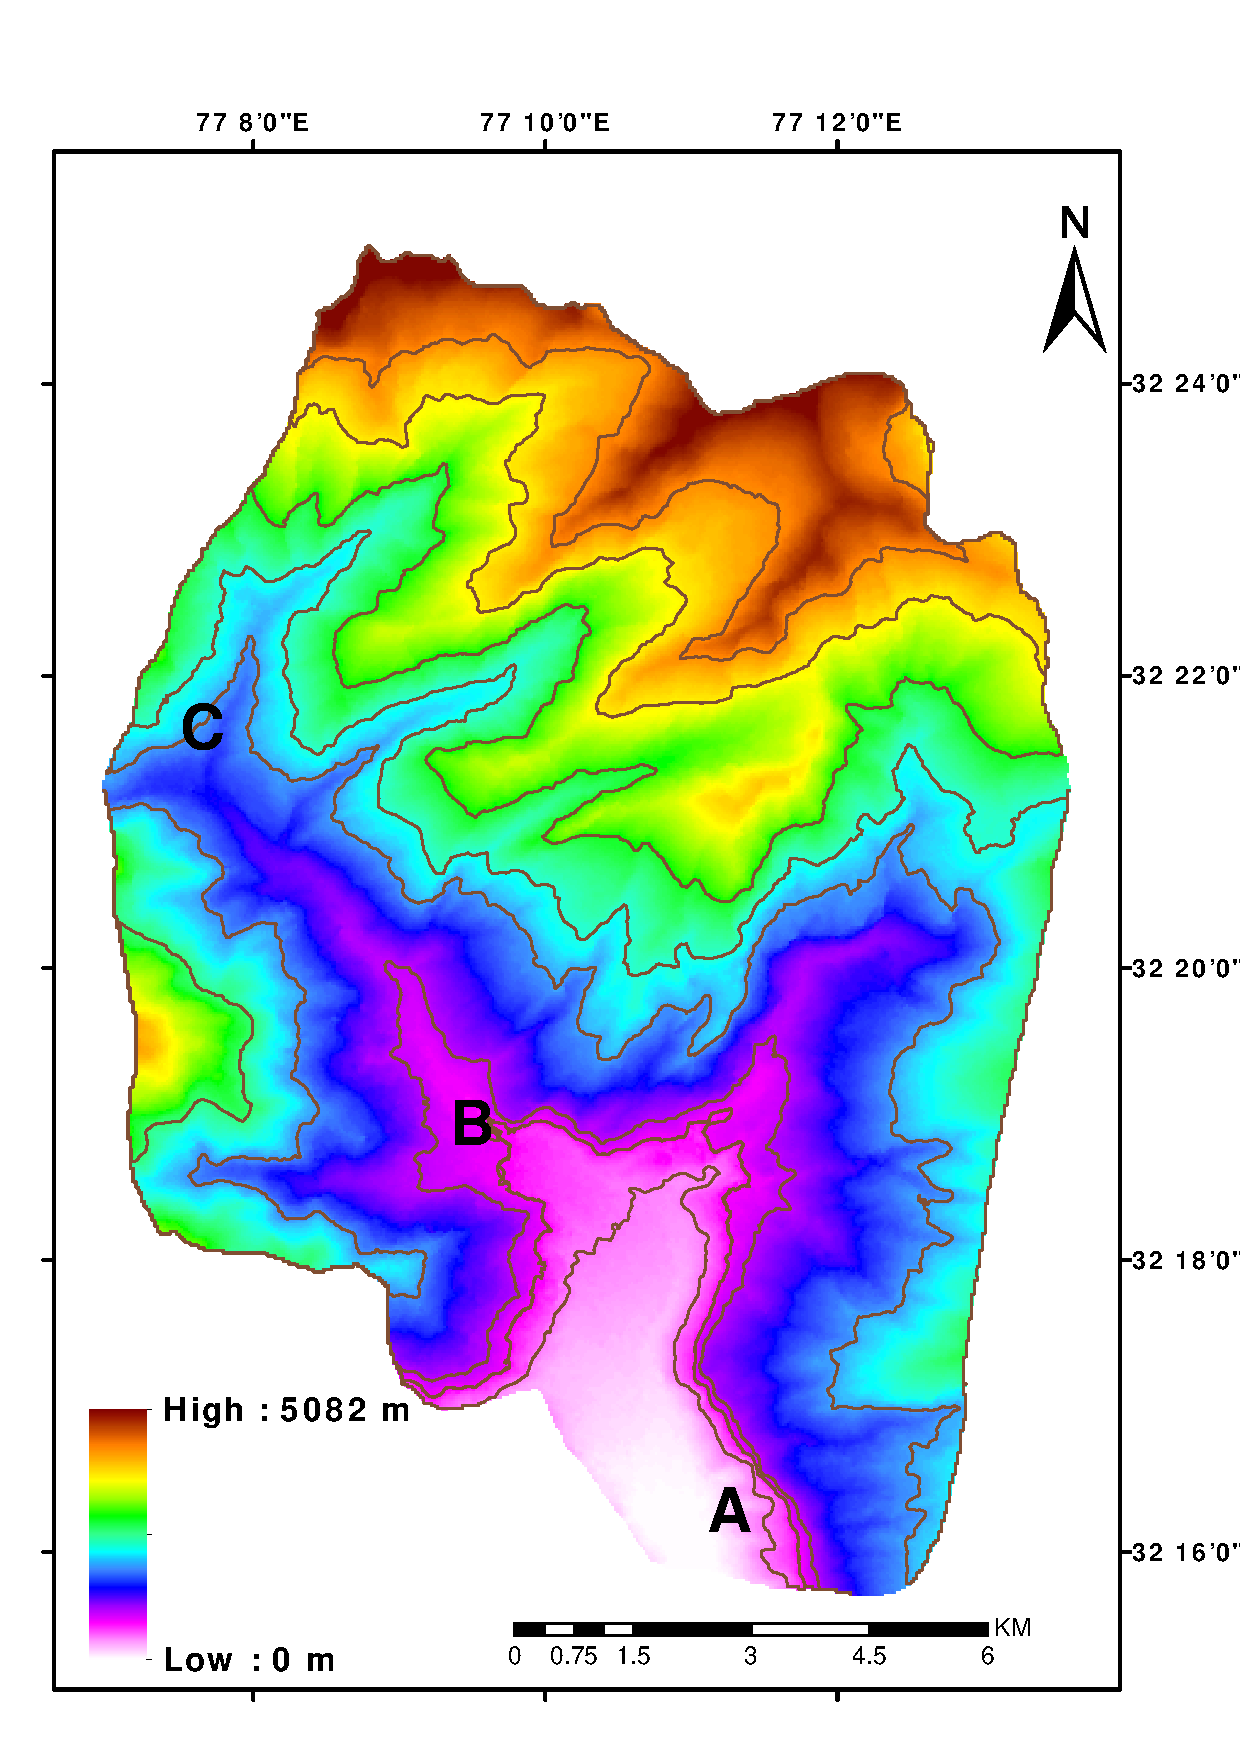
\includegraphics[width=0.45\columnwidth]{Figures_SSD/DEM_subset}} \hspace{1mm}
	\subfloat[]{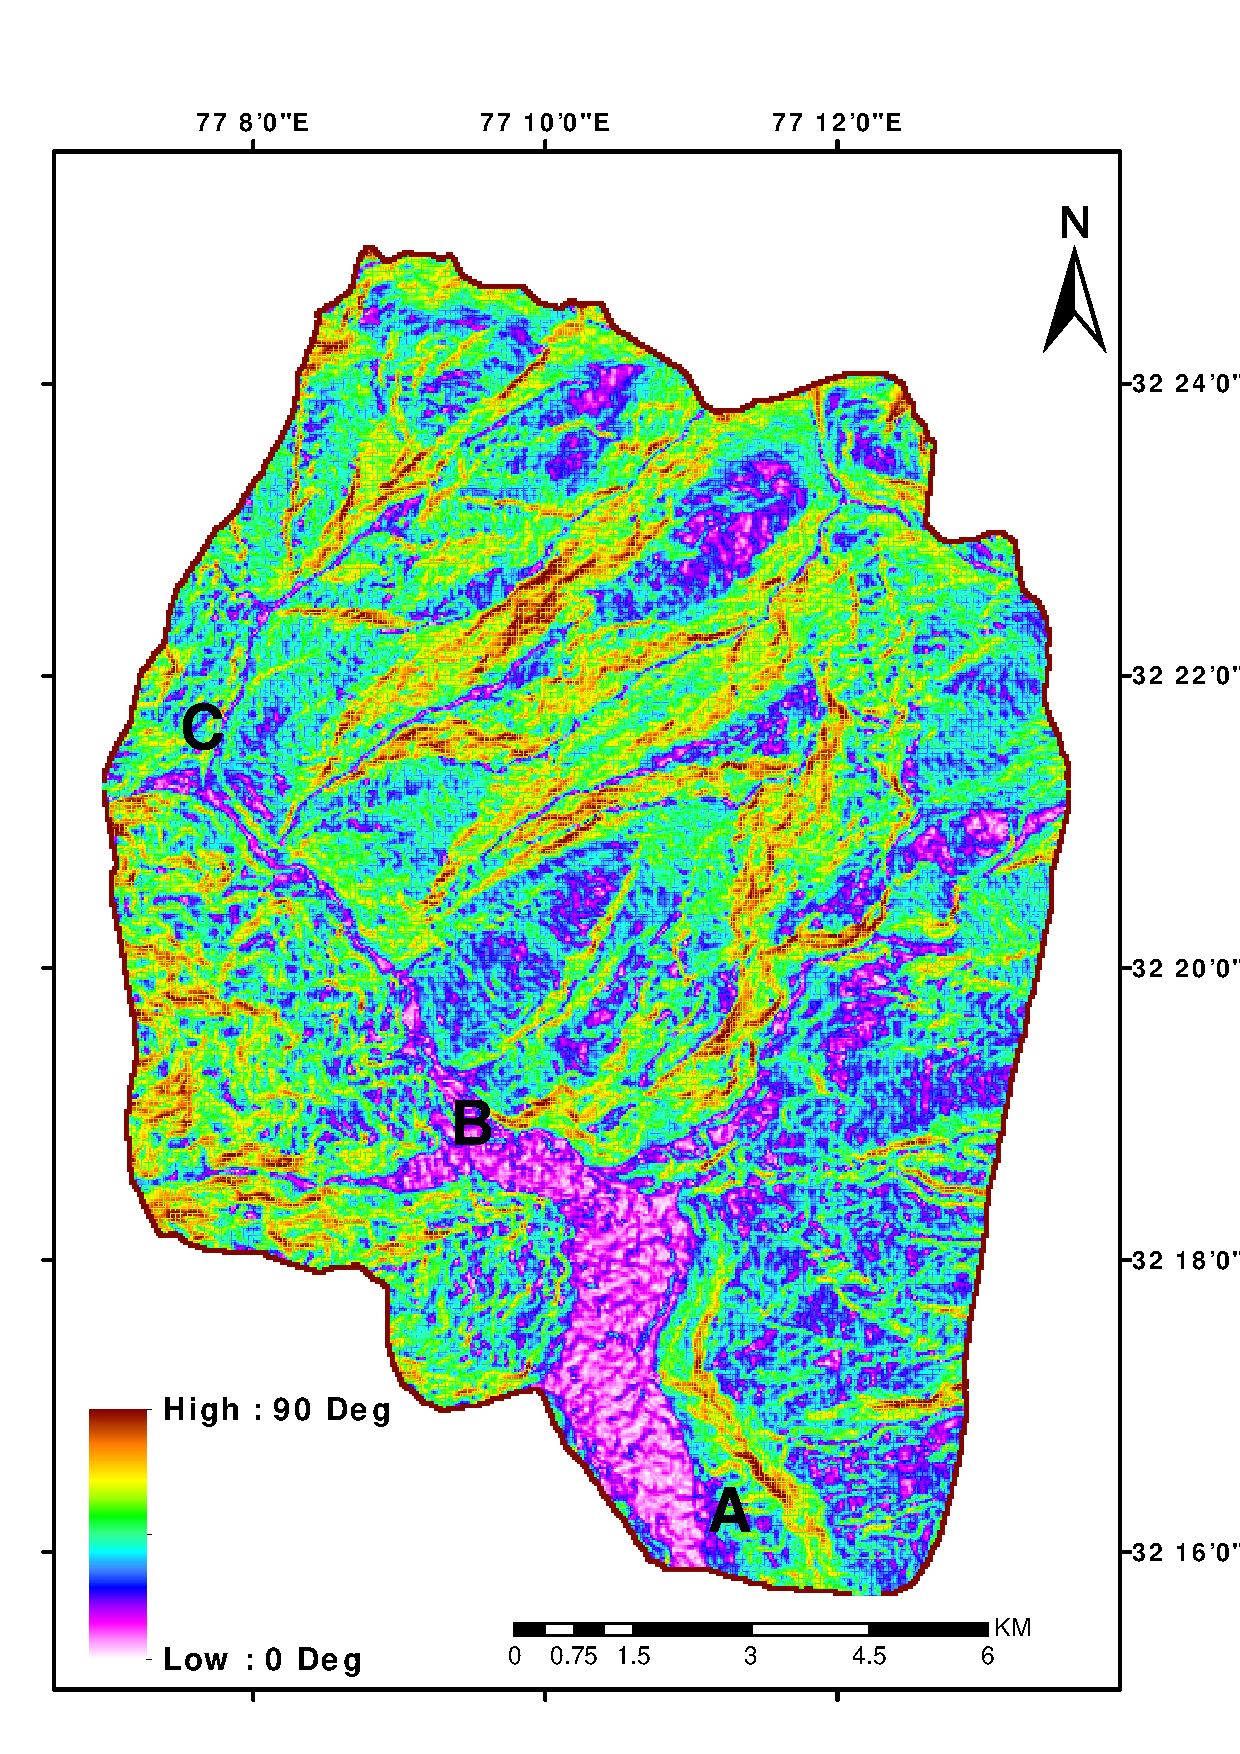
\includegraphics[width=0.45\columnwidth]{Figures_SSD/Slop}} \hspace{1mm}
	\subfloat[]{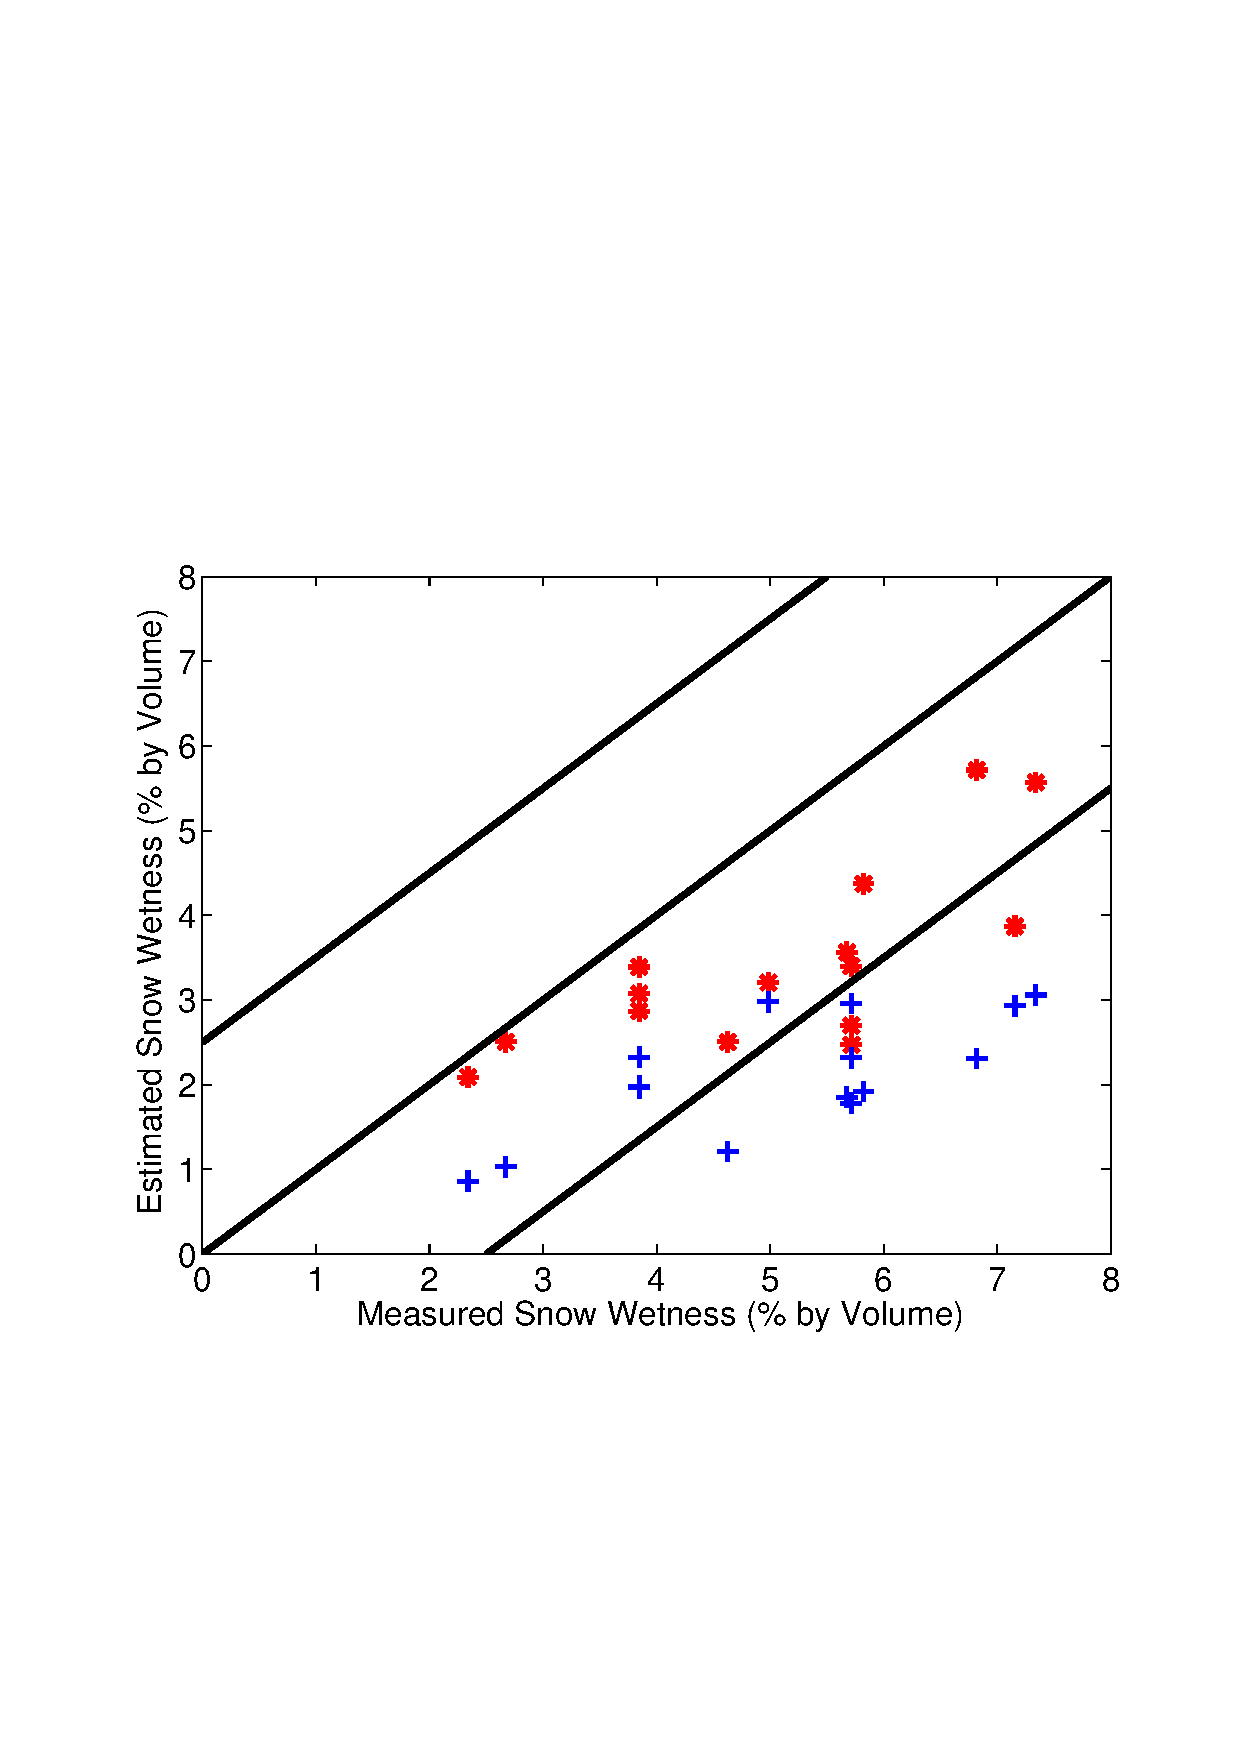
\includegraphics[width=0.65\columnwidth]{Figures_SSD/validation_plot.png}}
	\caption [SRTM 30~m DEM, Slope over the study area and validation plot]{(a). 30 m SRTM DEM and (b). slope map over the study area. (c). Validation Plot }
	\label{fig:DEM,Slope and Validation plot}
\end{figure*}

\begin{figure*}[!htbp]
	\centering
	\subfloat[]{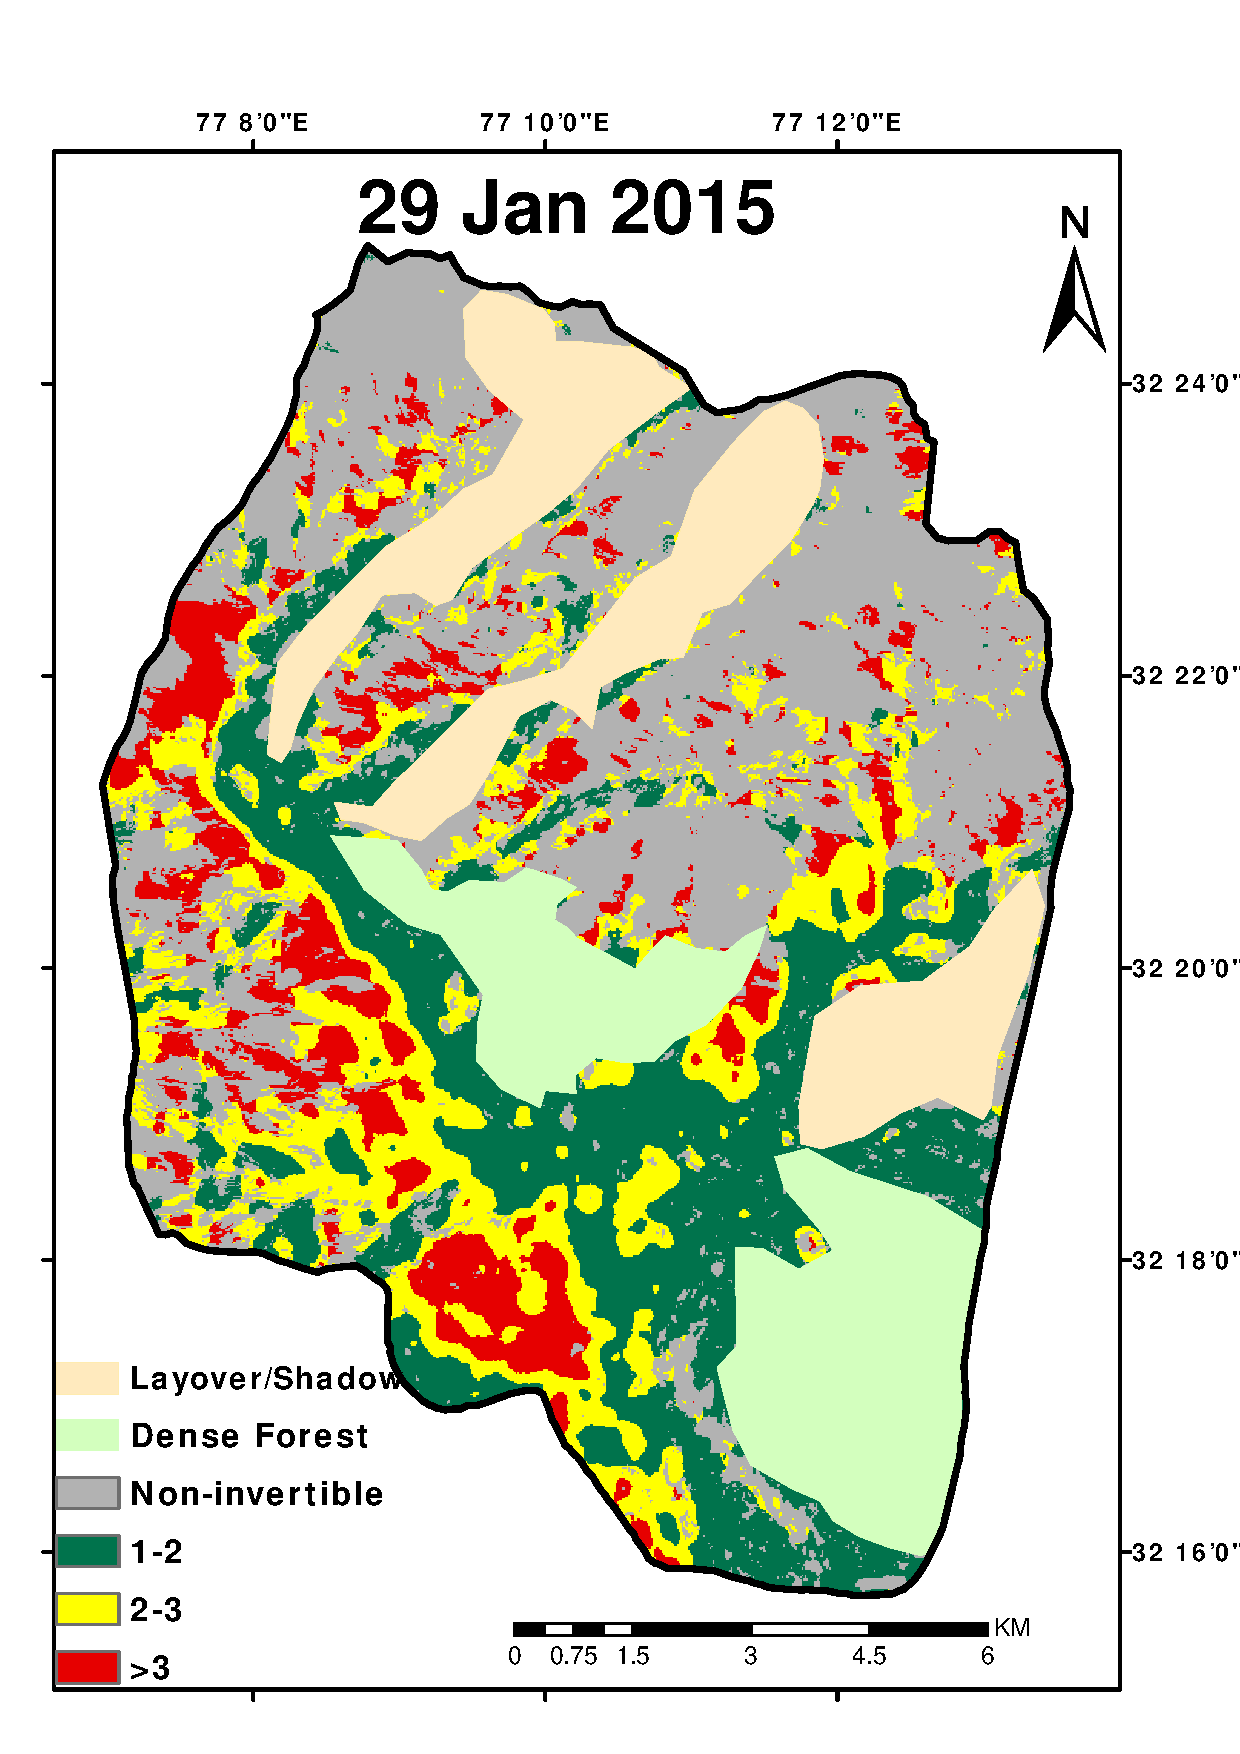
\includegraphics[width=0.45\columnwidth]{Figures_SSD/SSD_29Jan15}} \hspace{1mm}
	\subfloat[]{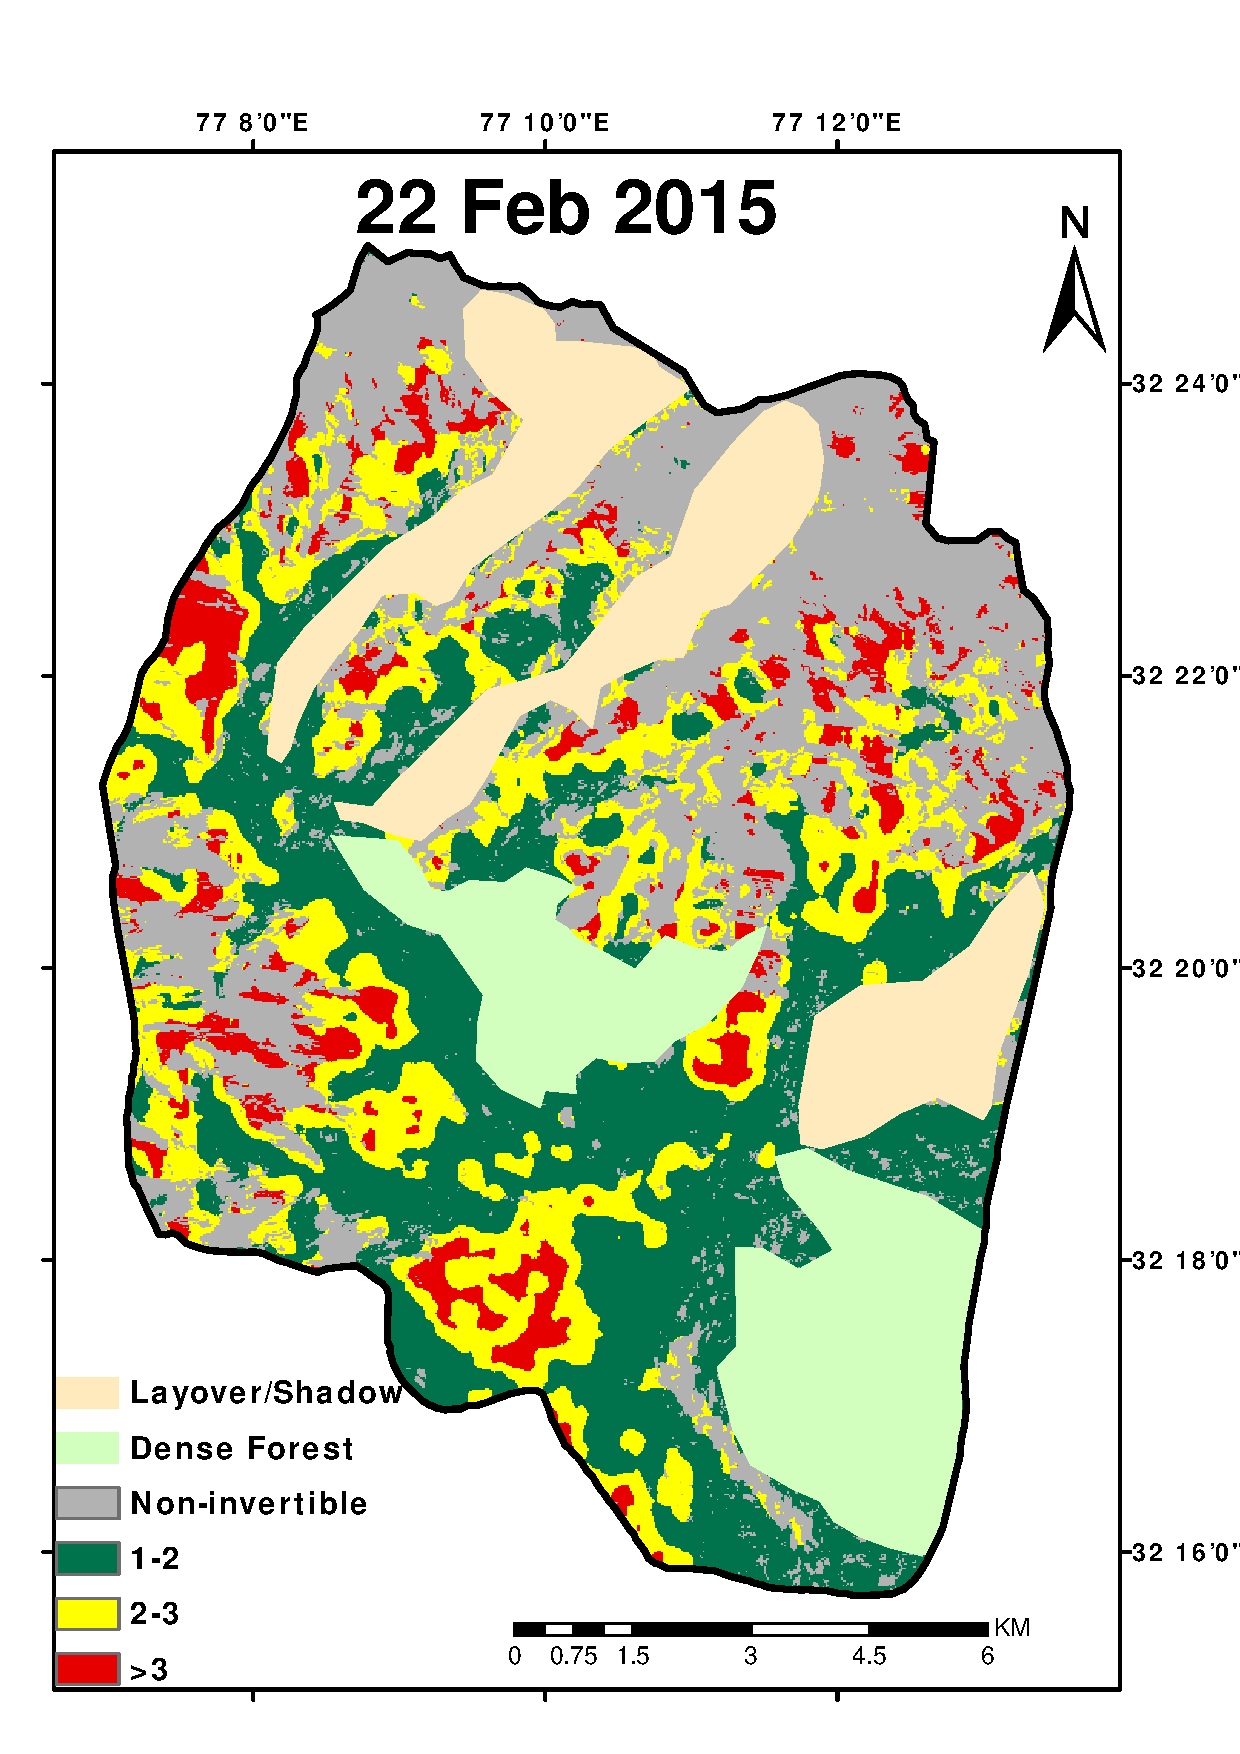
\includegraphics[width=0.45\columnwidth]{Figures_SSD/SSD_22Feb15}} 
	\hspace{1mm}
	\subfloat[]{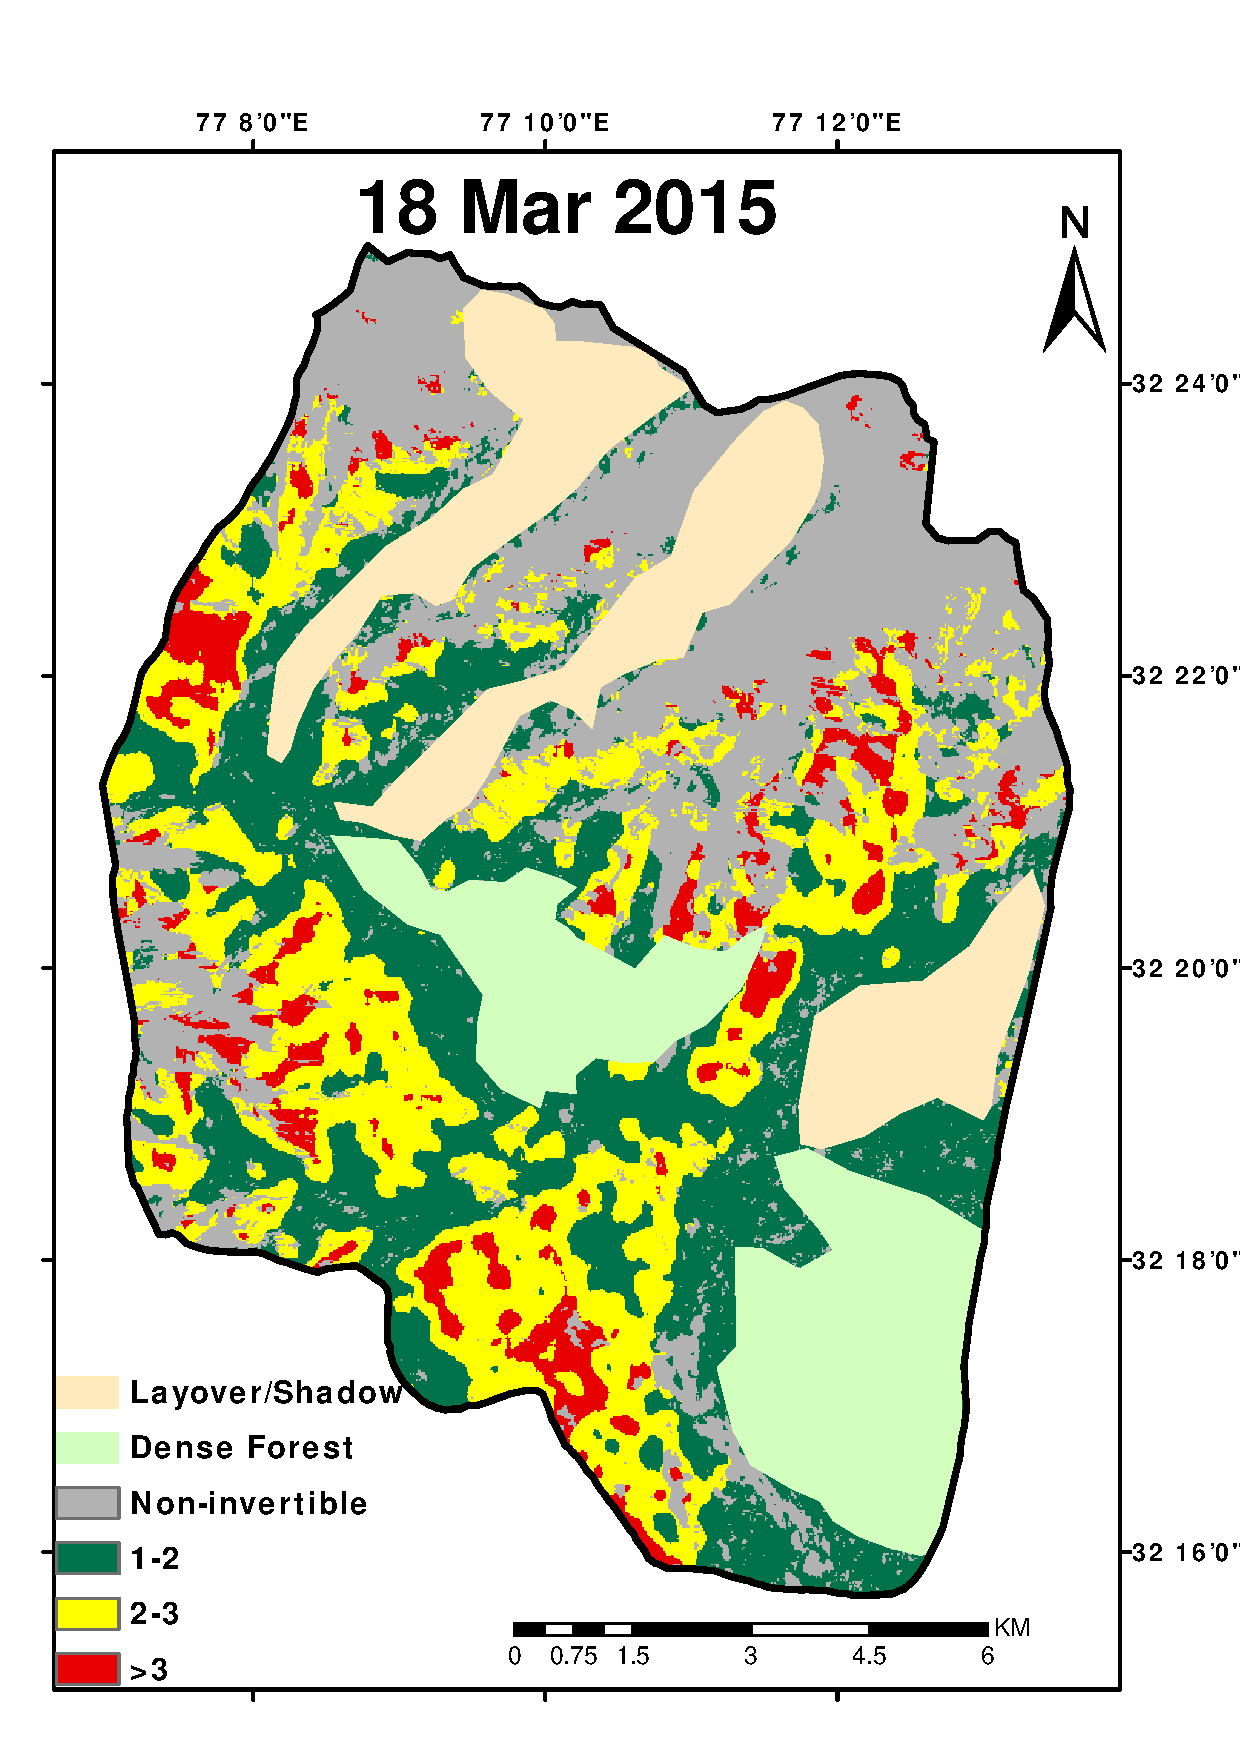
\includegraphics[width=0.45\columnwidth]{Figures_SSD/SSD_18Mar15}} 
	\caption[Multi-temporal snow surface dielectric constant maps]{Multi-temporal snow surface dielectric constant maps in a season over the study area. (RADARSAT-2 Data and Products ©MacDonald, Dettwiler and Associates Ltd. (2014) $--$ All Rights Reserved. RADARSAT is an official trademark of the Canadian Space Agency) }
	\label{fig:Multi_temporal_SSD}
\end{figure*}

The estimated snow surface dielectric constant maps for 7 Feb. 2012, 8 Feb. 2013 and 18 Feb. 2014 using the proposed algorithm are shown in Figure~\ref{fig:SSD_results}(a), ~\ref{fig:SSD_results}(b) and ~\ref{fig:SSD_results}(c) respectively. The points A, B and C on the maps indicate the observatory locations at Bahang, Solang and Dhundi which are at an altitude of 2006~m, 2446~m and 2896~m respectively. The percentage of areas covered with different snow surface dielectric constant ranges, for all the three data sets are presented in Table~\ref{table:SSD_range}. It is observed that in all the maps, the snow cover with the surface dielectric constant falling within the range of 2--3 are in most of the areas. Generally in the month of February, the snowfall with considerable temperature variation is observed over the Indian Himalayan region. This condition will initiate the melt-freeze process in the snowpack. 

On 7 Feb. 2012 the descending pass data was acquired around 6.18 AM IST (Indian Standard Time) along with the in-situ measurements collected around the Bahang observatory. The estimated surface dielectric constant values over the Bahang observatory are in the range of 1.5--2 which are closer to the measured values. It can be observed that around 18$\%$ of the area shows the surface dielectric constant values of $>$3. These are mostly over high altitudes along with high slopes (Figure~\ref{fig:DEM,Slope and Validation plot}(a) and Figure~\ref{fig:DEM,Slope and Validation plot}(b)). The Dhundi observatory shows more than 20~cm melting on 6 Feb. 2012. This melting rate might be higher over the slopes than the flat observatory areas. However, during the descending pass acquisition, the observed low temperature ($<-2^\circ$C) might have frozen the melted water over the snow surface within few centimeters. This frozen depth should be lower over the slopes compared to the flat areas. The observed high dielectric constant over the slopes is due to the presence of wet snow layers on the top of the snowpack. These conditions clearly distinguish the low surface dielectric constant over the flat areas and high over the slopes. High wetness and density values over the same slopes have been reported in~\cite{surendar2015snowwetness,surendar2015snowdensity} for the same dataset.

The dielectric constant map for 8 Feb. 2013 (Figure~\ref{fig:SSD_results}(b)) almost follows the same trend as compared to the previous year (7 Feb. 2012). The observed maximum temperature on 7 Feb. 2013 at Bahang, Solang and Dhundi were 11$^\circ$C, 7$^\circ$C and 6$^\circ$C with a melting of around 11~cm, 23~cm and 9~cm, respectively. However, the observed low temperature during the descending pass acquisition at Bahang ($-3^\circ$C), Solang ($-7.5^\circ$C) and Dhundi ($-7^\circ$C) have frozen the snowpack surface similar to the previous year. The snow surface dielectric constant map for the ascending pass data acquired on 18 Feb. 2014 at 6.30 PM IST is shown in Figure~\ref{fig:SSD_results}(c). The different range of values of dielectric constant with snow covered areas for 18 Feb 2014 is shown in Table~\ref{table:SSD_range}. It can be seen from the map (Figure~\ref{fig:SSD_results}(c)) that mostly the areas with high slopes on the eastern side show high dielectric constant range ($>$3). This is because of the direct sun's illumination on the eastern slopes during sunset just before the acquisition. 

Temporal variation of the snow surface dielectric constant map for a 2015 winter season is shown in Figure~\ref{fig:Multi_temporal_SSD}(a)--(c). The snow surface dielectric constant map for 29 Jan. 2015 data is shown in Figure~\ref{fig:Multi_temporal_SSD}(a). It can be observed that over the observatory locations the snow surface dielectric constant values are in the range of 1--2 and which are increasing over the low altitude slopes. This may be because of no fresh snowfall on 28 Jan. 2015 and the maximum temperature observed was 3$^\circ$C, 9.5$^\circ$C and 11$^\circ$C at Dhundhi, Solang and Bahang stations, which melts the snow surface considerably. But during the acquisition observed minimum temperature (-7$^\circ$C, -3.5$^\circ$C and -1.5$^\circ$C at Dhundhi Solang and Bahang observatories respectively) might have frozen the snow surface in few cm over flat observatory locations and which are low over the slope areas. But over high altitude regions the pixels are mostly non-invertible. This may be because of the fresh snowfall which produces dominant volume scattering mechanism.The total percentage of the invertible pixels for snow surface dielectric constant was around 30$\%$ for this data.  
%In the high altitude  over the observatory locations. The minimum temperature on that day were . Fresh snow fall was observed on Solang and Dhundhi observatories but no fresh snow fall on 28 Jan 2015. The maximum temperature observed was 3$^\circ$C, 9.5$^\circ$C and 11$^\circ$C at Dhundhi, Solang and Bahang stations, which melts the snow surface (the standing snow at all the three observatories were 158~cm, 90~cm and 12~cm respectively) But the minimum temperature frozen the melting water in few cm in flat observatory locations and which are low over the slop areas. 
\begin{table}[!htbp]
	\caption[Comparison of invertible pixels by both the optimization techniques]{Comparison of the percentage of area utilized for the snow surface dielectric constant inversion using the criteria for $(m_{E}^{\mbox{\scriptsize opt}})$ and $(p_{max})$. }
	\begin{center}
		\begin{tabular}{|c|c|c||c|c||c|c|} \hline
			Dielectric Range & \multicolumn{6}{c|}{Area ($\%$)} \\
			\cline{2-7}
			& \multicolumn{2}{c||}{7 Feb. 2012} & \multicolumn{2}{c||}{8 Feb. 2013} & \multicolumn{2}{c|}{18 Feb. 2014}\\
			\cline{2-7}
			& $m_{E}^{\mbox{\scriptsize opt}}$ & $ p_{max}$ & $m_{E}^{\mbox{\scriptsize opt}}$ & $p_{max}$ & $m_{E}^{\mbox{\scriptsize opt}}$ & $p_{max}$ \\ \hline
			1-2 &	13.77 & 13.91 & 17.03 & 17.61 & 17.54 & 18.21 \\ \hline
			2-3 &	24.44 & 25.30 & 25.26 & 26.37 & 19.93 & 21.04 \\ \hline
			$>$3&   18.31 & 18.90 & 11.91 & 12.64 & 17.53 & 17.86 \\ \hline
			\bf Total&  \bf 56.52 & \bf 58.11 & \bf 54.2 & \bf 56.52 & \bf 55.00 & \bf 57.11 \\ \hline \hline
			Dense forest cover & 12.59 &	12.59 &	12.59 & 12.59 & 12.59 & 12.59 \\ \hline
			Layover/Shadow & 12.67 & 12.67 & 12.67 & 12.67 & 15.42 & 15.42 \\ \hline
		\end{tabular}
	\end{center}
	\label{table:SSD_range}
\end{table}

The snow surface dielectric constant map for 22 Feb. 2015 is shown in Figure~\ref{fig:Multi_temporal_SSD}(b). There was no snowfall observed on 21 $\&$ 22 Feb. 2015 over the study area. As per the temperature fluctuation within a day snow started to melt and freeze. During the acquisition snow surface got frozen because of the low temperature. Since, there was no recent snowfall the top snow surface layers are wet which produces dominant surface scattering. So that, the total percentage of the invertible pixels for snow surface dielectric constant was around 40$\%$ for this data. For the data of 18 Mar. 2015, the snow surface dielectric constant (Figure~\ref{fig:Multi_temporal_SSD}(c)) was inverted for around 35 $\%$ of pixels which was lower than the 22 Feb 2015 data. This may be because of the observed fresh snowfall of 5~cm and 25~cm over Solang and Dhundhi regions on 17 March 2015.  Most of the higher altitude pixels are not invertible because of this fresh snowfall.

A total of 20 in-situ measurements were collected in near real time with the satellite data for the three consecutive years to validate the proposed snow surface dielectric constant estimation algorithm. The snow surface dielectric constant estimated by the proposed algorithm along with in situ measurements is plotted in Figure~\ref{fig:DEM,Slope and Validation plot}(c). The dielectric constant of top 5~cm of the snowpack is considered as the snow surface dielectric constant for validation of the proposed method. The correlation coefficient between the measured and the estimated snow surface dielectric constant is 0.95 at 95$\%$ confidence interval with a root mean square error (RMSE) of 0.20. The snow surface dielectric constant estimated from G4U based generalized surface parameter (~\cref{sec:3.2}) is compared with this proposed new method and validated using the in-situ measurements~(\ref{fig:comparision_of_SSD}). The correlation coefficient between the measured and the G4U based snow surface dielectric constant is 0.92 at 95$\%$ confidence interval with a root mean square error (RMSE) of 0.22.

\begin{figure*}[!htbp]
	\centering
	\includegraphics[width=0.6\columnwidth]{Figures_SSD/Comparision_plot} 
	\caption [Comparision of SSD]{Comparision of SSD estimated from $\alpha_{s1}$ and the G4U based method with the in-situ measurements }
	\label{fig:comparision_of_SSD}
\end{figure*}



%\begin{figure*}[!h]
%	\centering
%	\subfloat[\label{Fig:DEM}]{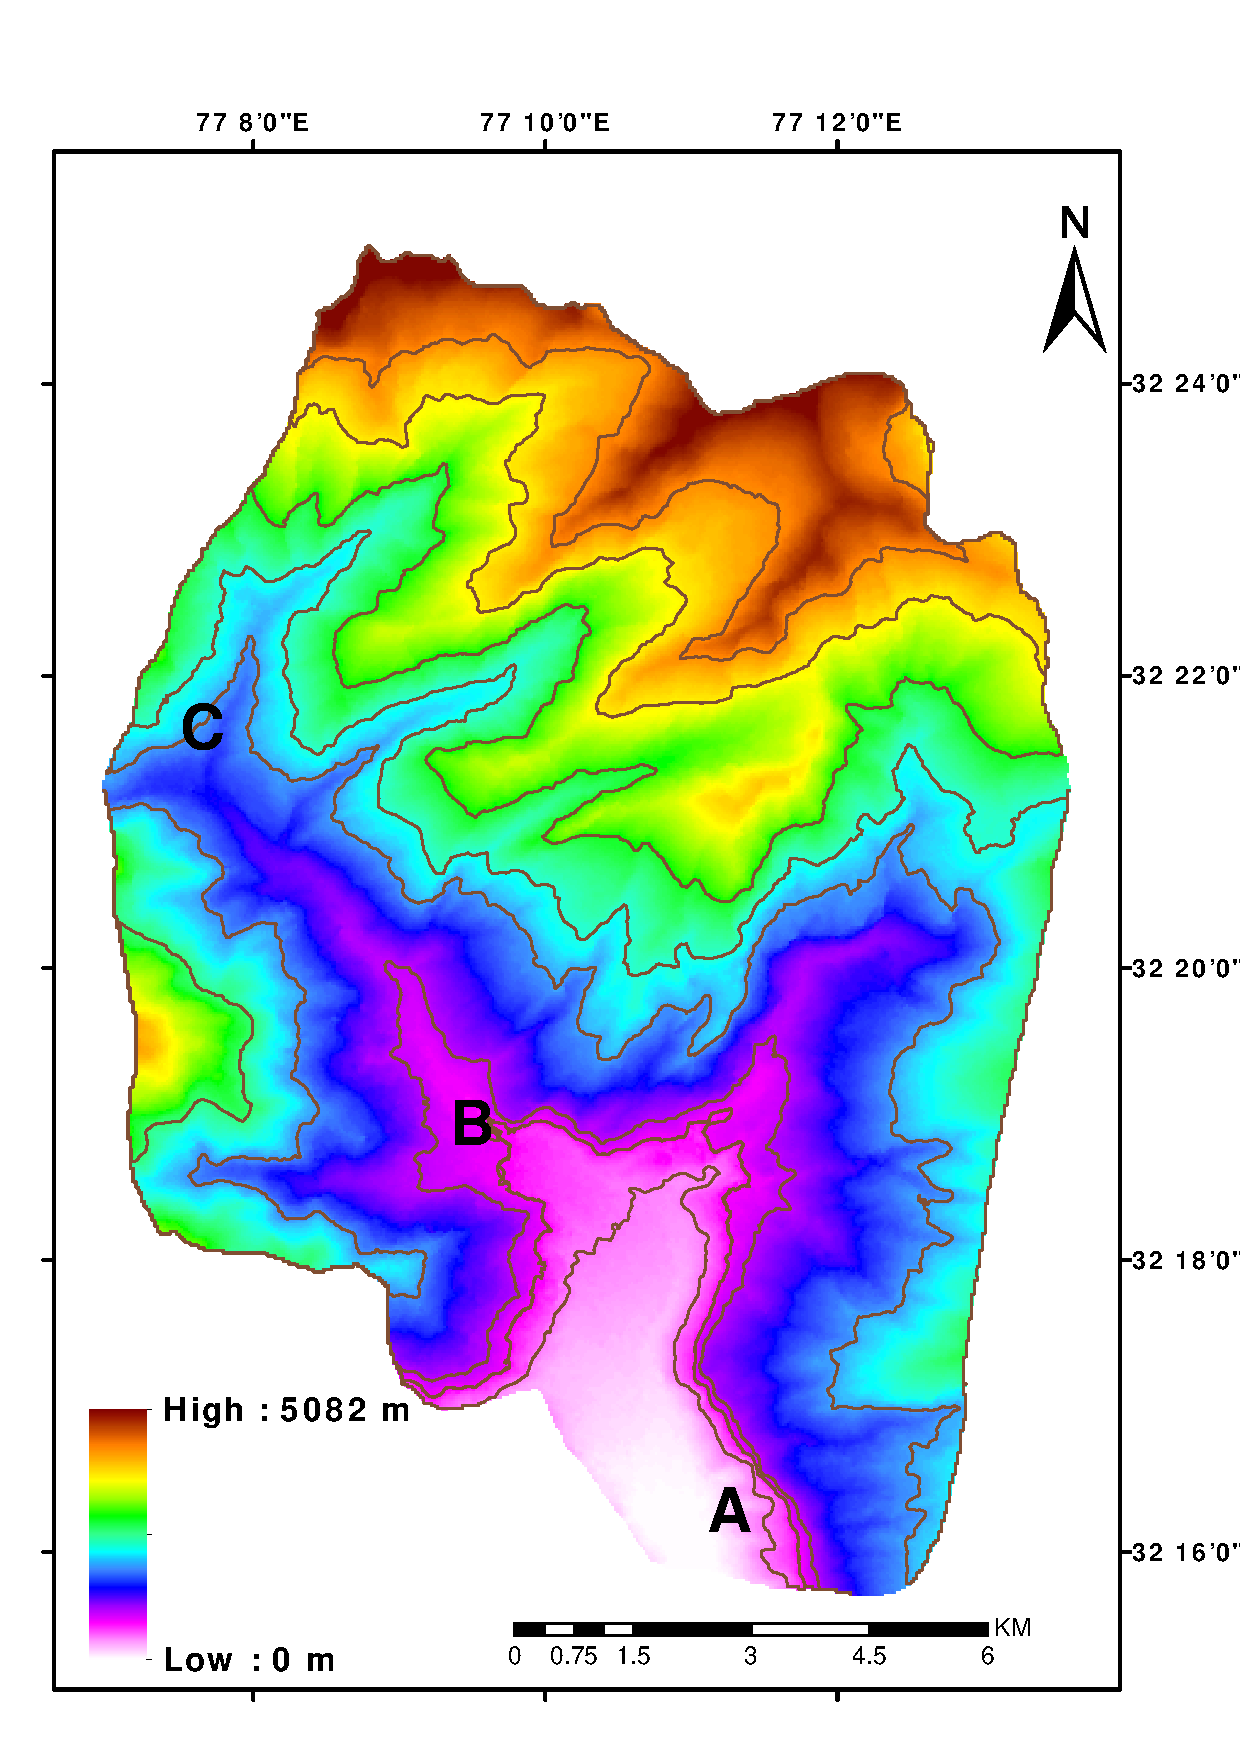
\includegraphics[width=0.4\columnwidth]{Figures_SSD/DEM_subset}} \hspace{1mm}
%	\subfloat[\label{Fig:Slop}]{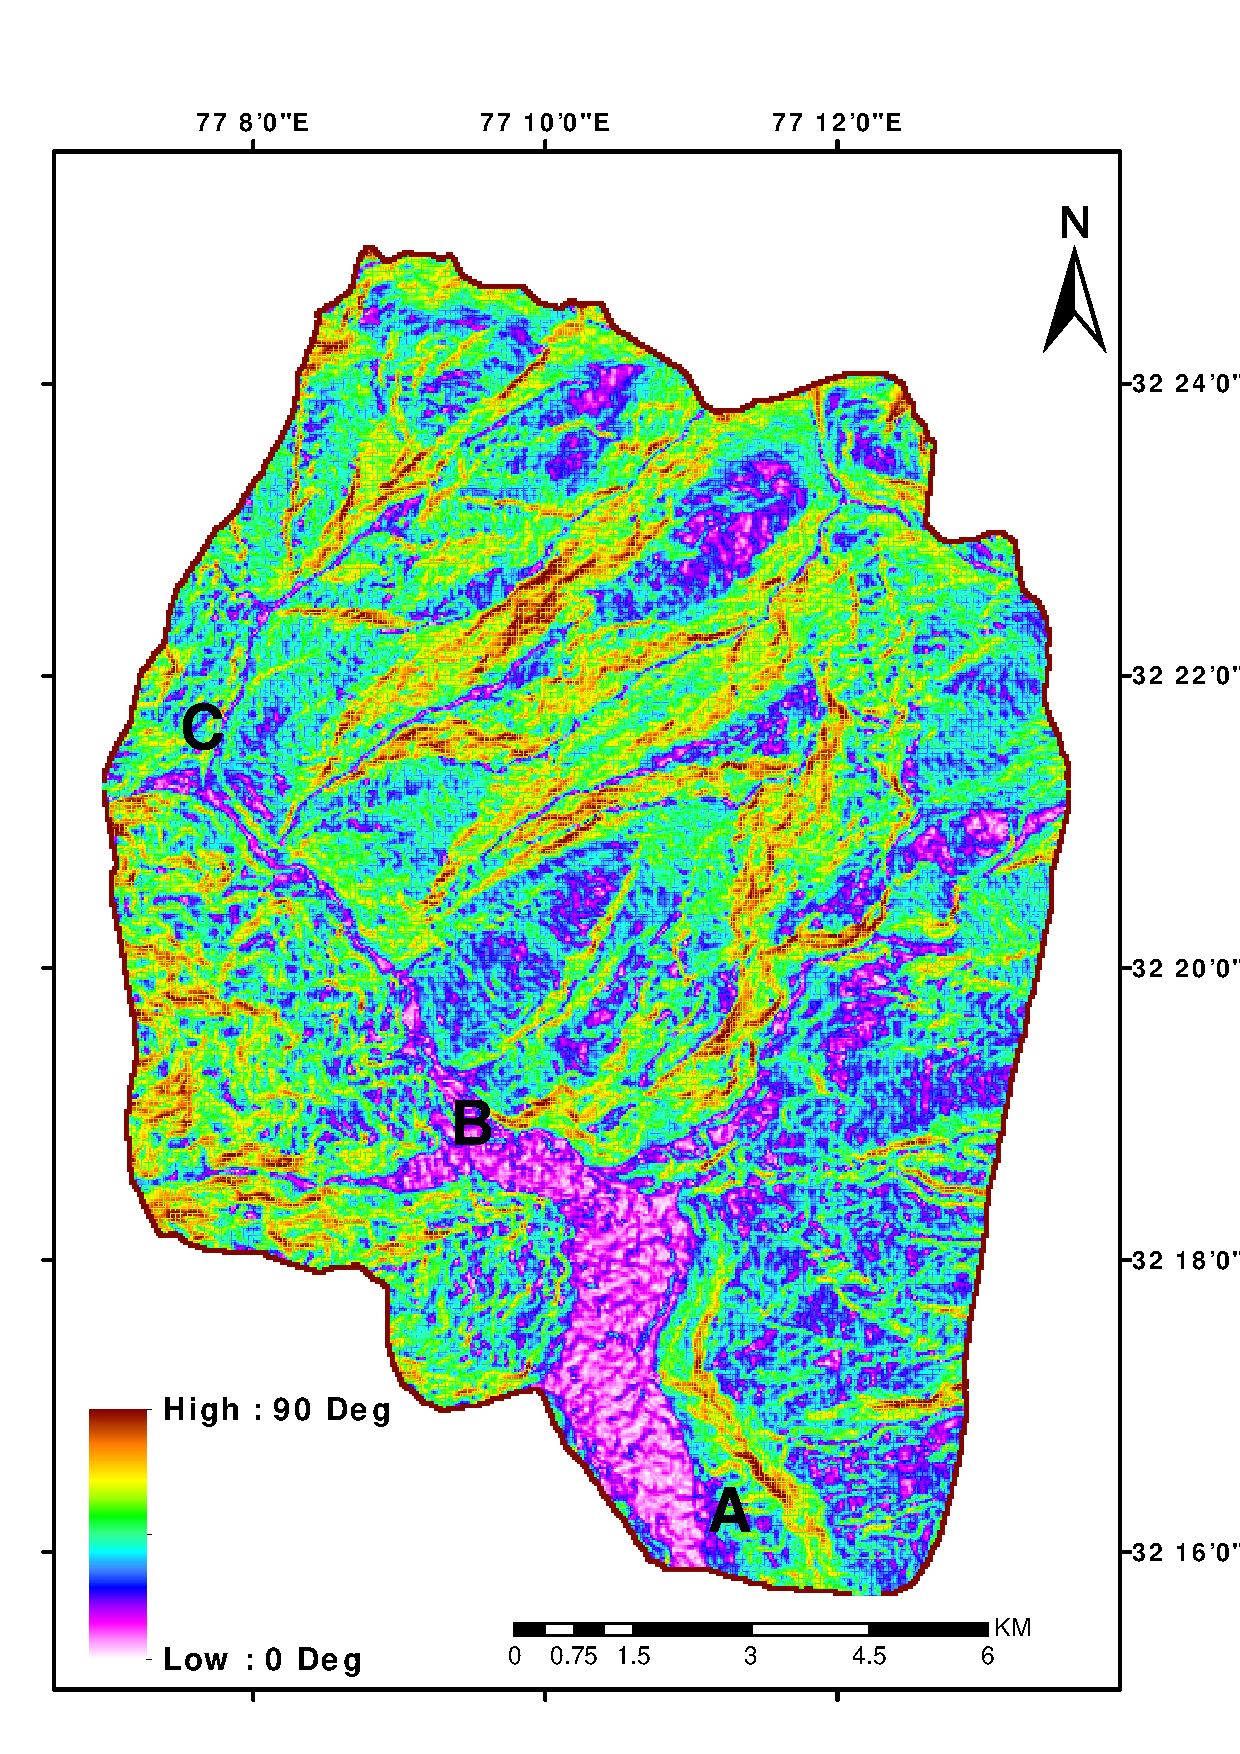
\includegraphics[width=0.4\columnwidth]{Figures_SSD/Slop}} \hspace{1mm}
%	\subfloat[\label{Fig:Validation_plot}]{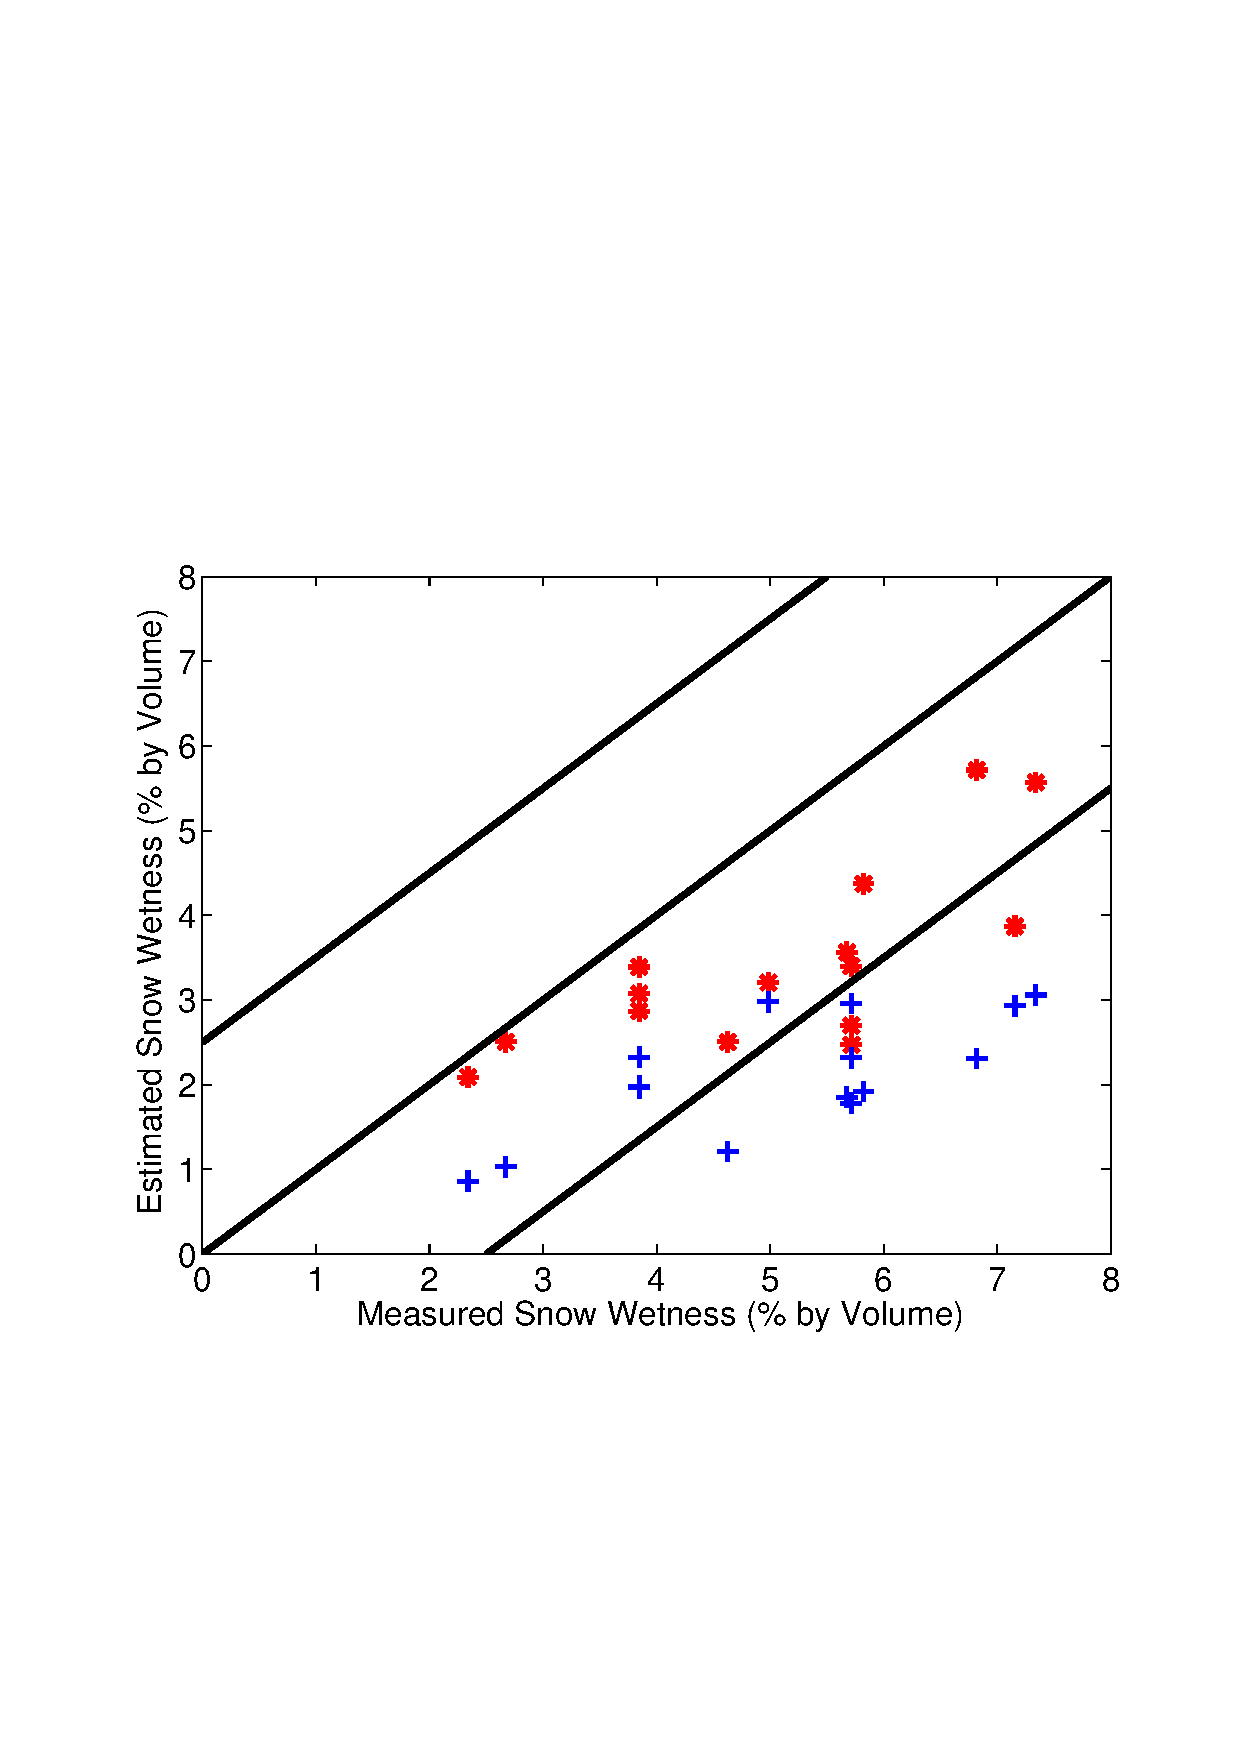
\includegraphics[width=0.65\columnwidth]{Figures_SSD/validation_plot.png}}
%	\caption{\protect\subref{Fig:DEM}. 30 m SRTM DEM and \protect\subref{Fig:Slop} slope map over the study area. \protect\subref{Fig:Validation_plot} Validation Plot }
%	\label{fig:results_3}
%\end{figure*}
\FloatBarrier
\section{Snow density}
\label{S:4}

In this section, the algorithm proposed in~\cref{sec:3.4} for the estimation of snow density from full polarimetric SAR data is analyzed using Radarsat-2 C-band SAR data. The results are analyzed over the study area explained in~\cref{sec:4.2.1}. The snow density estimated by the proposed method for 7 Feb. 2012 data is given in Figure~\ref{fig:proposed_results}(a). The range of 0.2--0.35~gcm$^{-3}$ density value occupies a maximum extent of about 46$\%$ of total study area (Table.~\ref{table:snow_density_range}). The observed density range in the map is possibly due to the increased grain size by the snowpack compaction. This is understood by studying the meteorological record at Dhundhi observatory (Figure~\ref{fig:multi_temp_plots}(a),(b)). From 6 to 7 Feb. 2012, the recorded temperature increased from 2$^\circ$C to 5$^\circ$C and wind speed of 2--4 km/hr, causing snow metamorphism. Also during this period the snowpack depth reduced by 33~cm as per the observatory data. Both the temperature and the wind speed together might have caused the reduction of snow depth and the compaction of the snowpack (~\citep{MET40}). In the map Figure~\ref{fig:proposed_results}(a), around 25$\%$ of the study area shows dense forest and geometric distortions (Table.~\ref{table:snow_density_range}). All the Radarast-2 descending pass data over this region possibly shows this distortions.

\begin{figure*}[!htbp]
	\centering
	\subfloat[]{\includegraphics[width=0.45\textwidth]{Figures_sd/7Feb2012}}
	\subfloat[]{\includegraphics[width=0.45\textwidth]{Figures_sd/8Feb2013}} \\
	\subfloat[]{\includegraphics[width=0.45\textwidth]{Figures_sd/18Feb2014}}
	\caption [Snow density mps from Radarsat-2 data]{Snow density maps derived from the proposed methodology. (For figure (c): RADARSAT-2 Data and Products ©MacDonald, Dettwiler and Associates Ltd. (2014) $-$ All Rights Reserved. RADARSAT is an official trademark of the Canadian Space Agency)}
	\label{fig:proposed_results}
\end{figure*}

\begin{table}[!htbp]
	\caption{Percentage of area with snow density range}
	\begin{center}
		\begin{tabular}{|c|c|c|c|} \hline
			Snow Density Range (gcm$^{-3}$) & \multicolumn{3}{c|}{Area $\%$} \\
			\cline{2-4}
			& 7 Feb. 2012 & 8 Feb. 2013 & 18 Feb. 2014 \\ \hline
			0.0--0.05 &	1.38 &	2.86 &	1.84 \\ \hline
			0.05--0.1 &	0.73 &	4.15 &	0.98 \\ \hline
			0.1--0.15 &	3.10 &	4.75 &	3.65 \\ \hline
			0.15--0.2 &	5.79 &	5.70 &	5.07  \\ \hline
			0.2--0.25 &	14.00 &	7.17 &	9.03 \\ \hline
			0.25--0.3 &	20.28 &	7.20 &	14.24 \\ \hline
			0.3--0.35 &	11.80 &	3.78 &	11.01 \\ \hline
			0.35--0.4 &	4.02 &	0.92 &	5.10 \\ \hline
			0.4--0.45 &	1.82 &	0.15 &	2.87 \\ \hline
			0.45--0.5 &	0.37 &	0.01 &	1.13 \\ \hline
			\hline		
			Dense forest cover &	12.59 &	12.59 &	12.59 \\ \hline
			Layover/Shadow &	12.67 &	12.67 &	15.42 \\ \hline
			Snow free/Wet snow &	11.42 &	38.06 &	17.06 \\ \hline
		\end{tabular}
	\end{center}
	\label{table:snow_density_range}
\end{table}


During the same period in the following year (8 Feb. 2013), the density was estimated in the range of 0.2--0.3~gcm$^{-3}$ as shown in Figure~\ref{fig:proposed_results}(b). This range of density values covers around 15$\%$ of the entire study area as shown in Table.~\ref{table:snow_density_range}. However, snow free/wet snow regions in the snow density map were around 38$\%$ as seen in Table.~\ref{table:snow_density_range}. This might be because of the maximum temperature recorded on 7 Feb. 2013. The observed temperatures at the Bahang, Solang and Dhundhi observatories on 7 Feb. 2013 were 11$^\circ$C, 7$^\circ$C and 6$^\circ$C (Figure~\ref{fig:multi_temp_plots}(c)), respectively which were higher than 2012. However, it can be observed that the snow density values are lower than the previous year (7 Feb. 2012). This may be because of the fresh snowfall on 6 Feb. 2013. Even though high temperature was observed on 7 Feb. 2013, the snowpack might not have compacted firmly during the acquisition on 8 Feb. 2013 as compared to the multiple melt-freeze condition in 2012. 

The estimated snow density map and the observatory measurements for the 18 Feb. 2014 data (Figure~\ref{fig:proposed_results}(c)), shows a similar trend as that of 7 Feb. 2012. Unlike the 7 and 8 Feb, the 18 Feb. 2014 data was acquired in an ascending pass. It can be seen in Table.~\ref{table:snow_density_range} that 34$\%$ of the area was covered with the snow density values in the range of 0.2--0.35~gcm$^{-3}$. There was no fresh snowfall recorded for a week prior to the acquisition on 18 Feb. 2014. Moreover, a large variation can also be observed between the maximum and the minimum temperatures on 18 Feb. 2014 (Figure~\ref{fig:multi_temp_plots}(d)). So the old snowpack has undergone multiple melt-refreeze process, which has increased the snowpack grain size and consequently, the snow density. 

\begin{figure*}[!htbp]
	\centering
	\subfloat[]{\includegraphics[width=0.49\textwidth]{Figures_sd/Temp_variability_jan_2015}}
	\subfloat[]{\includegraphics[width=0.49\textwidth]{Figures_sd/Temp_variability_feb_2015}} \\
	\subfloat[]{\includegraphics[width=0.49\textwidth]{Figures_sd/Temp_variability_mar_20151}} 
	\caption [Temperature variation plots]{Temporal variation of average local temperature over the study area in (a) Jan 2015; (b) Feb 2015; (c) March 2015 (the data were taken from the site:http://www.accuweather.com as on 17 April 2015)}
	\label{fig:temp_plots_2015}
\end{figure*}

\begin{figure*}[!htbp]
	\centering
	\subfloat[]{\includegraphics[width=0.49\textwidth]{Figures_sd/Temp_variability_2012}} \hspace{0.1cm}
	\subfloat[]{\includegraphics[width=0.49\textwidth]{Figures_sd/windspeed_variability_2012}} \\
	\subfloat[]{\includegraphics[width=0.49\textwidth]{Figures_sd/Temp_variability_observatories_2013}}\hspace{0.1cm} 
	\subfloat[]{\includegraphics[width=0.49\textwidth]{Figures_sd/Temp_variability_observatories_2014}} 	
	\caption[Temperature and windspeed variation over Dhundhi observatory]{(a) Temporal variation of temperatures over Dhundhi in Feb. 2012; (b) Temporal variation of wind speed over Dhundhi in Feb. 2012; (c)-(d) Temporal variation of minimum and maximum temperatures over all the three observatories in Feb 2013 and 2014 respectively}
	\label{fig:multi_temp_plots}
\end{figure*}

The Radarsat-2 data acquired with the same geometry on 29 Jan, 22 Feb and 18 Mar. 2015 was used to analyze the snow density changes within a season. The snow density map of 29 Jan 2015 (Figure~\ref{fig:multi_temp_density}(a)) indicates that the study area was completely covered with fresh snow. The estimated snow density values are less than 0.1 gcm$^{-3}$ in most of the areas as shown in Figure~\ref{fig:multi_temp_density}(a). Generally, by the end of January, high amount of snow precipitation occurs in the Indian Himalaya. This is reflected in the map with low snow density values. The local averaged temperature plot (Figure~\ref{fig:temp_plots_2015}(a)), shows that the temperature drops to 4$^\circ$C during the acquisition day. This is the lowest temperature recorded during that particular week which may be because of fresh snowfall on that day. 

\begin{figure*}[!htbp]
	\centering
	\includegraphics[width=0.9\textwidth]{Figures_sd/temporal_variability_SD}
	\caption[Multi temporal snow density maps] {Temporal variation of snow density in a season. (RADARSAT-2 Data and Products ©MacDonald, Dettwiler and Associates Ltd. (2014) $--$ All Rights Reserved. RADARSAT is an official trademark of the Canadian Space Agency)}
	\label{fig:multi_temp_density}
\end{figure*}

The estimated snow density values were more than 0.2 gcm$^{-3}$ for most of the study area on 22 Feb. 2015, as shown in Figure~\ref{fig:multi_temp_density}(b). Normally in February, snowfall occurs and large variations between the minimum and the maximum temperatures were observed within a day. Hence, considerable melting and refreezing occurs in the snowpack which increases the snow density. As observed in Figure~\ref{fig:temp_plots_2015}(b), the averaged local temperature before the acquisition day was recorded at 12$^\circ$C. So, the snow surface melt might have refrozen during the descending pass acquisition (6.14 AM local IST). 

Snow density map of 18 Mar. 2015 shows that $>$ 0.3 gcm$^{-3}$ of snow density values are observed in most of the study area which is high as compared to the snow density map of February. Normally in March, the snowfall stops and the snowpack starts to melt. The white areas in this map (non-invertible pixels) possibly represents wet snow. This can be attributed to high temperature (Figure~\ref{fig:temp_plots_2015}(c)) which may have melted the snow surface so it causes the absence of snowpack volume scattering.

\begin{figure*}[!htbp]
	\centering
	\includegraphics[width=0.5\textwidth]{Figures_sd/snow_density_validation}
	\caption [validation plot of snow density algorithm]{Comparison of the snow densities estimated by the proposed methodology and in-situ measurements.}
	\label{fig:validation_plot}
\end{figure*} 

A total of 23 near-real time in-situ measurements were collected with the satellite data for three consecutive years to validate the proposed snow density estimation algorithm. The snow densities estimated by the proposed methodology and measured in the field are plotted in Figure~\ref{fig:validation_plot}. The mean absolute error (MAE) of  the proposed method is 0.027~gcm$^{-3}$ and the root mean square error (RMSE) is 0.032~gcm$^{-3}$. 



